%% V3.0
%% 2026/16/04

\documentclass[openacc]{rsproca_new}%%%%where rsproca is the template name
%TC:incbib
%Add here your packages or commands
% \usepackage{lipsum}
% \usepackage{multicol}
% \usepackage{natbib}

\addbibresource{refs.bib}

\usepackage{graphicx, float} %package to manage images
\graphicspath{ {figures/} }
\usepackage{mathtools}
\usepackage{float}
\newcommand{\bs}[1]{\boldsymbol{#1}}
\usepackage[dvipsnames]{xcolor}
\usepackage{booktabs}
\usepackage{array} % Required for the column shortcut
\usepackage{tabularx}
% --------------------------------------------------------------------------
% this is just for editing purpose; change it later
% \usepackage[colorinlistoftodos]{todonotes}

% https://www.overleaf.com/learn/latex/Questions/Can_I_add_inline_or_margin_comments_to_the_pdf%3F
% Use
% \todo[inline]{Here's an inline comment below the title \& author.}
% \listoftodos[A list of things I need to finish]

% Your abstract.\todo{You can use \textit{italic in a comment}, like this.}
% \todo[inline, color=red!50]{Inline todonotes.}%
% --------------------------------------------------------------------------------
%%%% *** Do not adjust lengths that control margins, column widths, etc. ***

%%%%%%%%%%% Defining Enunciations  %%%%%%%%%%%
\newtheorem{theorem}{\bf Theorem}[section]
\newtheorem{condition}{\bf Condition}[section]
\newtheorem{corollary}{\bf Corollary}[section]
%%%%%%%%%%%%%%%%%%%%%%%%%%%%%%%%%%%%%%%%%%%%%%%

\jname{rsif}
\Journal{J R Soc Interface\ }

\begin{document}

%%%% Article title to be placed here
\title{Predicting Unobserved Driver of Regime Shifts in Social-Ecological Systems With Universal Dynamic Equations}
% Predicting regime shifts in socio-ecological systems using scientific machine learning
% Predicting harvest rate as an unobserved parameter in a dynamical system undergoing regime shift.

\author{%%%% Author details
Kunal J. Rathore$^{1}$, John H. Buckner$^{1}$, Zechariah D. Meunier$^{1}$, Jorge Arroyo-Esquivel$^{2}$, James R. Watson$^{1}$}

%%%%%%%%% Insert author address here
\address{$^{1}$College of Earth, Ocean, and Atmospheric Sciences, Oregon State University, Corvallis, Oregon, USA\\
$^{2}$California Department of Fish and Wildlife, West Sacramento, California, USA}

%%%% Subject entries to be placed here %%%%
\subject{Ecology, Complex systems, social-ecological systems, Machine Learning, Regime Shifts, Non-linear dynamics}

%%%% Keyword entries to be placed here %%%%
\keywords{harvest rate, nonlinear dynamics, regime shift, population dynamics, neural networks, UDE, scientific ML}

%%%% Insert corresponding author and its email address}
\corres{Kunal Rathore\\
\email{rathorek@oregonstate.edu}}

%%%% Abstract text to be placed here %%%%%%%%%%%%
\begin{abstract}
   Ecosystems around the world are anticipated to undergo regime shifts as temperatures rise and other climatic and anthropogenic perturbations erode the resilience of present-day states. Forecasting these nonlinear ecosystem dynamics can help stakeholders to prepare for the associated rapid changes. One major challenge is that regime shifts can be difficult to predict when they are driven by unobserved factors. In this paper, we advance scientific machine learning methods, specifically universal dynamic equations (UDEs), to identify changes in an unobserved bifurcation parameter and predict ecosystem regime shifts. We demonstrate this approach using simulated data created from a dynamic model of a species population experiencing loss due to unobserved extraction or harvest. This could be, for example, illegal fishing from a fishery or unreported poaching in a game reserve. We show that UDEs can accurately identify changes in the unobserved bifurcation parameter, in our case the slowly increasing harvest rate, and predict when a regime shift might occur. Compared to alternative forecasting methods, our UDE approach provides competitive short-term predictions. This approach provides a new set of methods for ecosystem stakeholders and managers to identify unobserved changes in key parameters that drive nonlinear change.
\end{abstract}

%%%%%%%%%%%%%%%%%%%%%%%%%%%

%%%%%%%%%% Insert the texts which can accomdate on firstpage in the tag "fmtext" %%%%%

\begin{fmtext}
\section{Introduction}   

Human activities around the world are exerting increasing pressure on ecosystems. These impacts can be amplified by biological feedback mechanisms, leading to large and abrupt changes in the state of ecosystems called regime shifts \cite{scheffer2001catastrophic}. Ecological regime shifts can reduce the provision of ecosystem services, including carbon storage, biodiversity, and the maintenance of local climates, with cascading effects on food and water resources. These transitions, often driven by unobserved or nonlinear dynamics, can occur abruptly and intensify socioeconomic vulnerability by disrupting ecosystem services and livelihoods \cite{staver2011,turner2020climate, Biggs2018}. Understanding and forecasting the state of complex human-environmental systems becomes necessary if resource managers are to maximize economic benefits while preventing irreversible shifts. 

\end{fmtext}
%%%%%%%%%%%%%%% End of first page %%%%%%%%%%%%%%%%%%%%%

\maketitle
% \begin{multicols}{2}
\newpage

Ecological forecasting can provide ecosystem stakeholders and policymakers vital actionable information on how to adapt to changing environmental conditions \cite{dietze2017ecological, dietze2024near}. Predictive models play a crucial role in ecological forecasting, as they can help us to understand and prepare for often large and abrupt changes in ecosystem states \cite{clark2001ecological, kickert1999predictive, griffith2014new}. Examples include predicting species population dynamics in response to climate change \cite{urban2016improving}, forecasting harmful algal blooms for effective water resource management \cite{anderson2012progress}, and estimating wildfire risk based on vegetation and atmospheric conditions \cite{abatzoglou2016impact}. However, one major challenge in ecological forecasting is accounting for unobserved drivers of change. This is a common problem in many scientific domains such as epidemiology, where asymptomatic carriers and unreported cases alter the dynamics of disease transmission \cite{fraser2004factors}; economics, where latent variables such as consumer confidence impact macroeconomic outcomes \cite{stock2016dynamic}; and neuroscience, where unobserved neural states influence observed behavior and brain activity patterns \cite{paninski2010new}. This challenge is particularly critical when the unobserved quantity is a bifurcation parameter that governs rapid and large shifts in the qualitative properties of ecosystem dynamics. 

% Here, we consider populations that exhibit regime shifts caused by a hidden source of loss, such as illegal harvest from a fishery or poaching from a game reserve. In these systems, the harvest rate can be a bifurcation parameter \cite{may1976bifurcations} leading to unanticipated regime shifts. In such a scenario, an ecosystem with high abundance biomass (i.e., a stable regime, Fig. \ref{fig:scurve} Regime I) could pass through a transient regime (i.e., a flickering regime, Fig. \ref{fig:scurve} Regime II) to low biomass (i.e., the second stable regime, Fig. \ref{fig:scurve} Regime III). This presents an extreme challenge for ecosystem managers because these hidden drivers can push systems past critical thresholds without warning, often resulting in sudden ecosystem collapse that occurs too rapidly for conventional management interventions to prevent \cite{scheffer2009early, biggs2009turning}. Forecasting methods that identify the unobserved parameters could improve forecasting accuracy, improving the management of ecosystems as they undergo rapid changes.

Here, we consider populations that exhibit regime shifts caused by a hidden source of loss, such as illegal harvest from a fishery or poaching from a game reserve. In these systems, the harvest rate can be a bifurcation parameter \cite{may1976bifurcations} leading to unanticipated regime shifts. In such a scenario, an ecosystem with high abundance biomass (i.e., a stable regime, Fig. \ref{fig:scurve} Regime I) could pass through a transient regime (i.e., a flickering regime, Fig. \ref{fig:scurve} Regime II) to low biomass (i.e., the second stable regime, Fig. \ref{fig:scurve} Regime III). This presents a significant challenge for ecosystem managers: in systems where the bifurcation parameter is unobserved or poorly monitored, the proximity to a critical threshold may go unrecognized until a transition is already underway \cite{scheffer2009early, biggs2009turning}. While empirical evidence for abrupt, externally-driven regime shifts remains limited to a relatively small number of well-documented cases \cite{scheffer2009early}, theory suggests that hidden drivers of loss are particularly difficult to account for under conventional monitoring frameworks. Forecasting methods that identify the unobserved parameters could therefore improve early warning and management of ecosystems as they approach critical transitions.


\begin{figure}[h]
    \centering
    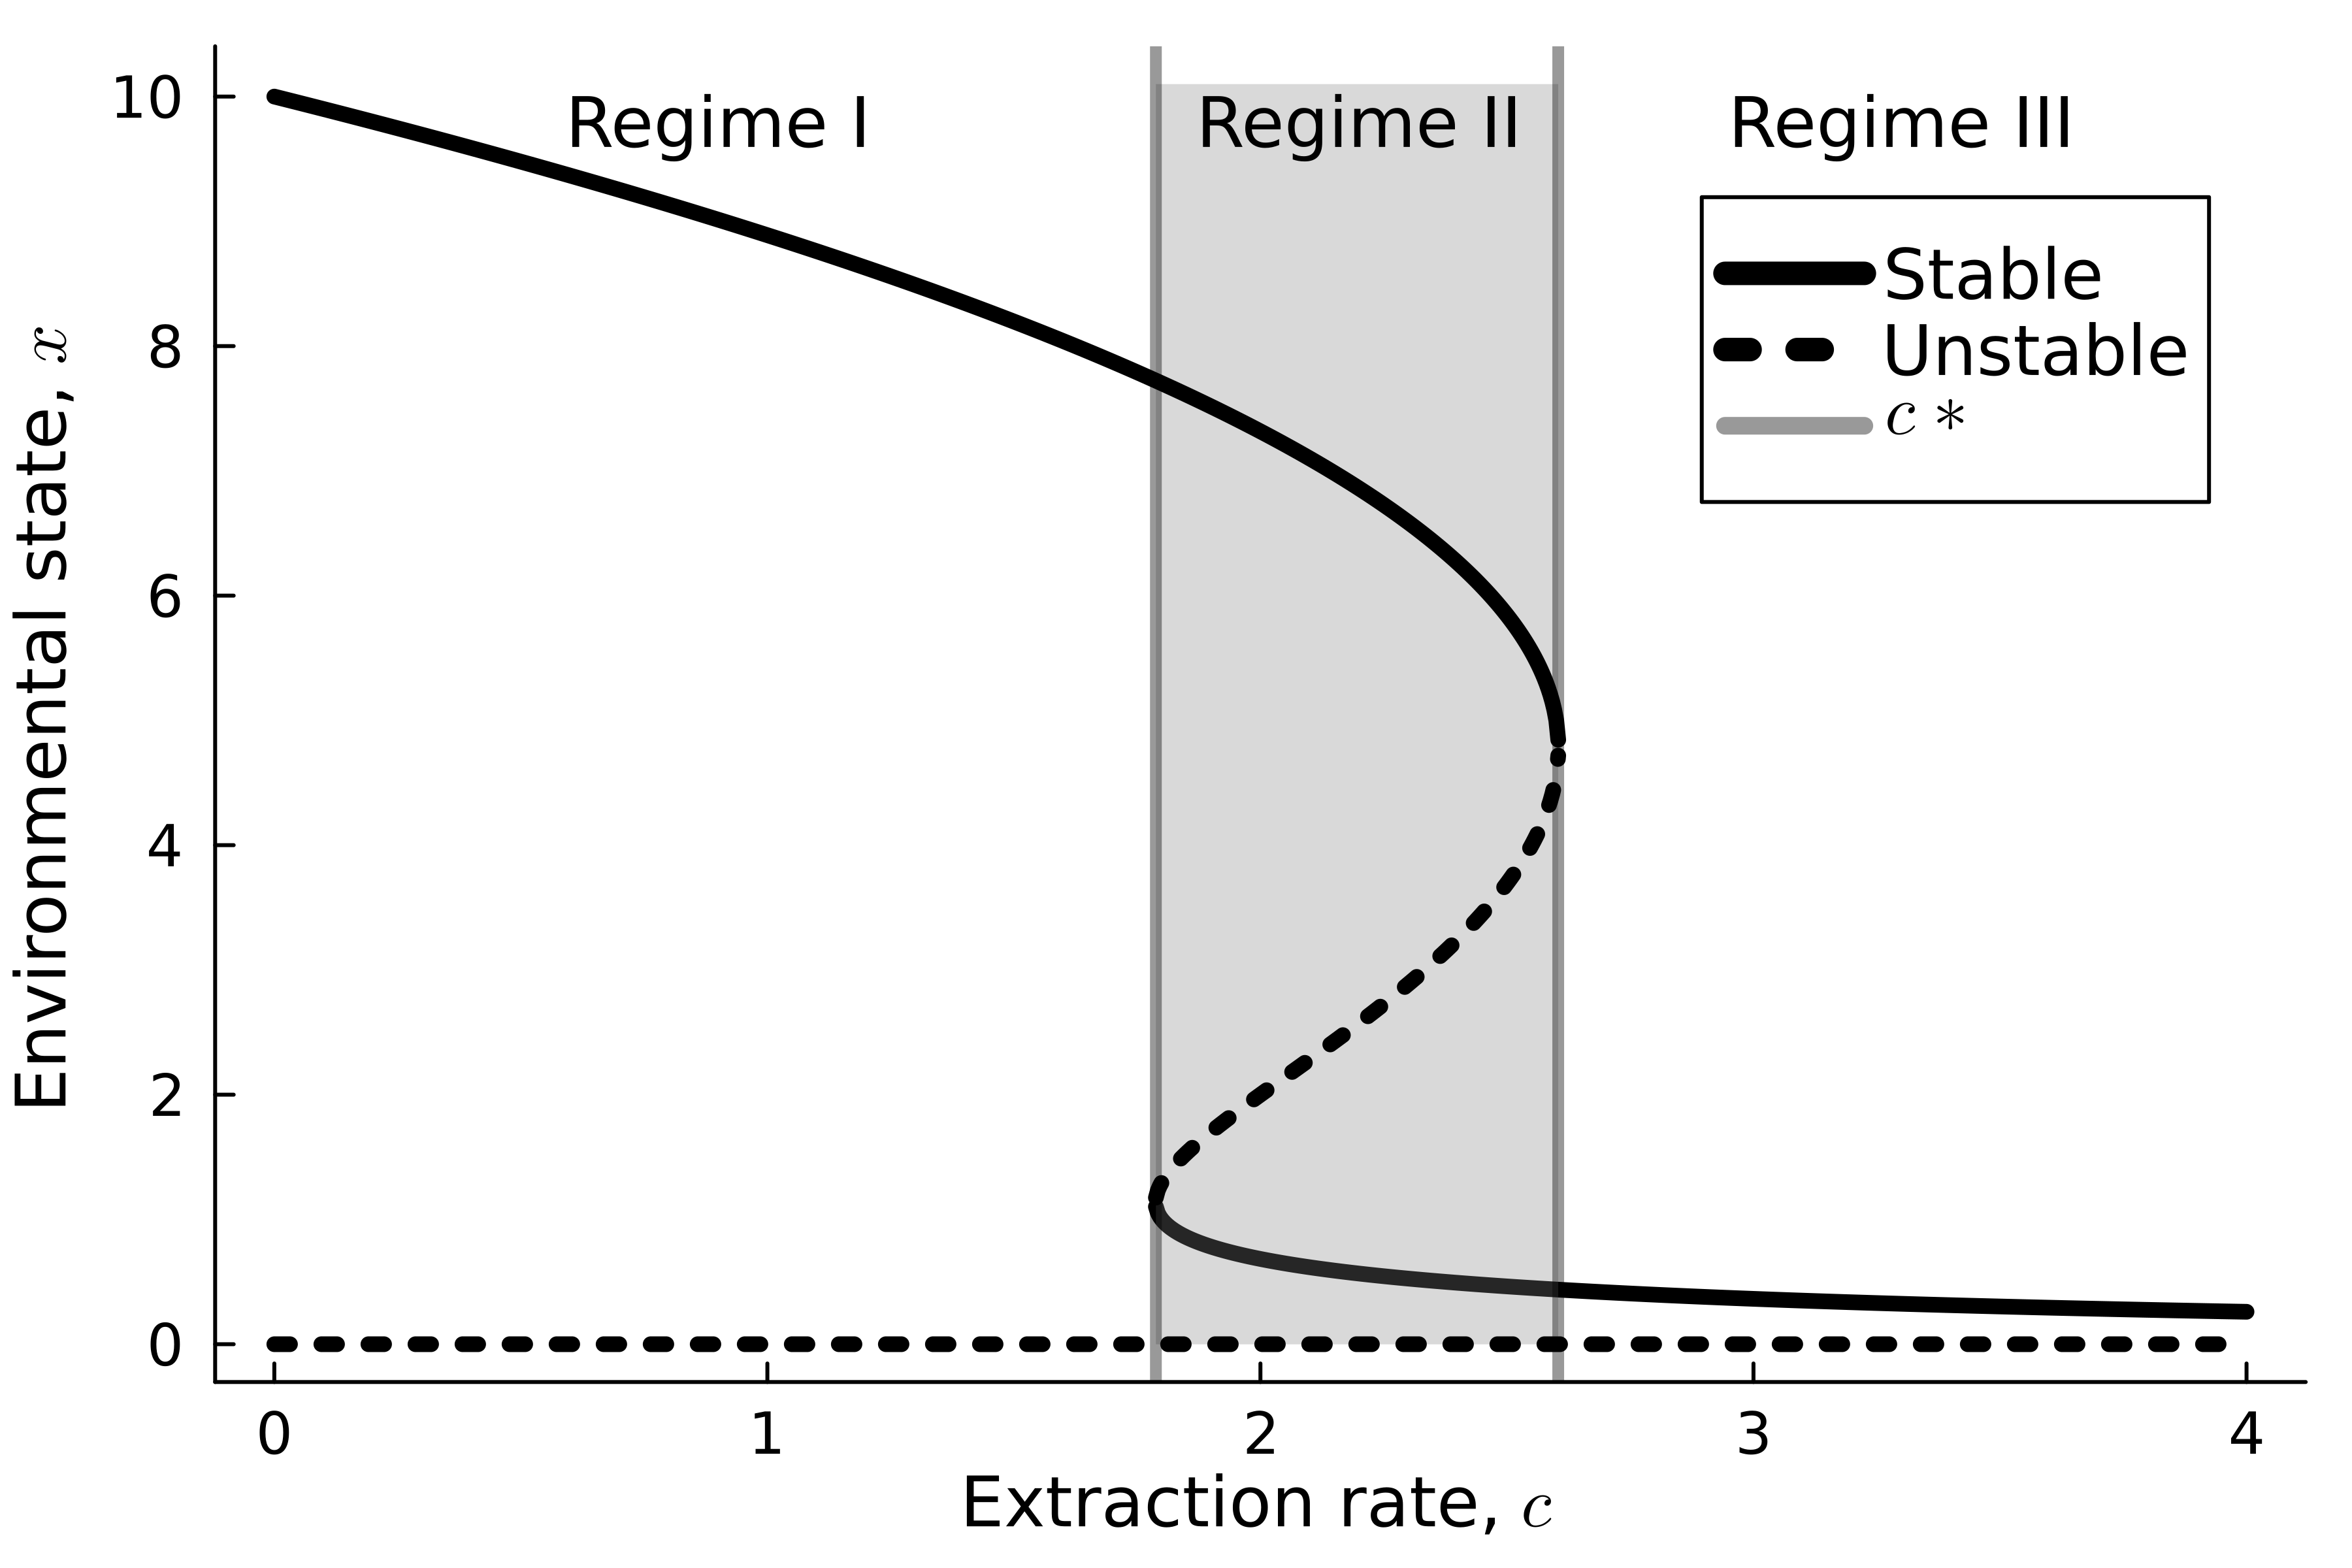
\includegraphics[width=0.5\linewidth]{figures/scurve.png}
    \caption{Bifurcation diagram illustrating the existence of three regimes in the deterministic dynamical system, where environmental state $x$ is a function of the harvest rate $c_t$. Solid splines indicate stable states, and dotted splines show unstable states. Vertical lines mark the regime boundaries at the equilibrium harvest rates $c*$ with regime II (shaded box) exhibiting bistability. Modified from \textcite{Tilman2024}}
    \label{fig:scurve}
\end{figure}

% A wide variety of mathematical and computational methods have been developed to forecast ecosystem regime shifts, including approaches based on dynamical systems, machine learning, and statistical modeling  
While early efforts to predict regime shifts relied on statistical modeling, recent advancements have increasingly integrated machine learning and, more critically, the formalisms of dynamical systems \cite{dakos2015resilience, ghadami2022data, PhysRevResearch.6.043194}.
Dynamical models are key tools for forecasting regime shifts, as they offer a framework for predicting critical transitions between stable states in ecosystems based on an explicit representation of key processes. These models use discrete-time difference and continuous-time differential equations to represent the underlying mechanisms driving the dynamics of the system, allowing researchers to identify early warning signals of tipping points and to improve our understanding of why these changes occur \cite{barnosky2012approaching, kefi2014early}. By formally representing interactions among system components and their responses to external perturbations, dynamical models offer information on the conditions that precipitate abrupt changes, such as shifts in ecosystem states, climatic patterns, or disease outbreaks \cite{biggs2015principles, may1977thresholds}.

Despite their relevance, these models have notable limitations when it comes to forecasting regime shifts. The parametrization process in dynamical models is crucial, but it can be challenging because multiple parameter sets can produce dynamics that are consistent with the data. In addition, the complexity of ecological systems characterized by numerous abiotic and biotic components, as well as direct and indirect interactions, introduces significant uncertainty in the predictions of dynamical models \cite{Dietze}. Furthermore, the functional forms embedded in these models, such as the choice of growth functions or predator-prey interaction terms, are often selected for mathematical tractability or historical convention rather than empirical support, and may inadequately represent the nonlinear dynamics that govern regime shifts \cite{clark2001ecological}. These models are also prone to overfitting (as are most models), especially with sparse or high-dimensional data, and struggle with the uncertainty and stochastic nature of ecological processes \cite{turchin2013complex}.


% In contrast, data-driven ``equation-free" methods are also commonly used to make ecological forecasts. They differ from equation-based approaches in that they do not rely on predefined functional forms or assumptions about the underlying processes. One such approach, empirical dynamical modeling (EDM), uses time series data to reconstruct and infer system dynamics without assuming explicit equations \cite{sugihara, perretti2013, Munch2024}. In addition, numerous machine learning approaches have been developed to provide predictions of ecosystem dynamics. Advanced neural network (NN) architectures, such as the recurrent neural network (RNN) and long short-term memory (LSTM) models, have shown great potential in overcoming the limitations of traditional equation-based methods \cite{Hochreiter}. However, the lack of mechanistic interpretability in these methods remains a key drawback that limits their broader applicability \cite{lipton2015}. Similarly, by not having explicit functional forms, these equation-free approaches often overlook valuable mechanistic insights that could improve forecasts, particularly when data are limited or have observation biases \cite{perretti2015estimating, Greff_2017}.

In contrast, data-driven ``equation-free'' methods are also commonly used to make ecological forecasts. They differ from equation-based approaches in that they do not rely on predefined functional forms or assumptions about the underlying processes. One such approach, empirical dynamical modeling (EDM), uses time series data to reconstruct and infer system dynamics without assuming explicit equations \cite{sugihara, perretti2013, Munch2024}. Recent extensions of EDM have further demonstrated its capacity to anticipate both the timing and type of critical transitions in nonlinear systems, as well as to detect regime shifts in chaotic dynamics and high-dimensional ecosystems \cite{grziwotz2023, huang2024, garain2025}. Despite these advances, purely equation-free methods remain limited in their ability to incorporate known mechanistic structure. An early attempt to bridge this gap was Wood's \citeyear{wood2001} framework of \textit{partially specified ecological models}, which replaced unknown interaction terms with flexible nonparametric functions while retaining the mechanistic skeleton of a dynamic model demonstrating that embedding data-driven flexibility within a mechanistic structure can improve both model fit and ecological interpretability \cite{wood2001}. In addition, several machine learning approaches have been developed to provide predictions of ecosystem dynamics. Advanced neural network architectures, such as the recurrent neural network and long short-term memory models, have shown great potential in overcoming the limitations of traditional equation-based methods \cite{Hochreiter}. However, the lack of mechanistic interpretability in these methods remains a key drawback that limits their broader applicability \cite{lipton2015}. Similarly, by not having explicit functional forms, these equation-free approaches often overlook valuable mechanistic insights that could improve forecasts, particularly when data are limited or have observation biases \cite{perretti2015estimating, Greff_2017}. Together, these limitations motivate the need for hybrid frameworks that can embed data-driven flexibility within a mechanistic structure---a principle now formalized through Universal Differential Equations (UDEs).


\begin{figure*}
    \centering
    % \fbox{\rule{0pt}{2in} \rule{0.9\linewidth}{0pt}}
    
\includegraphics[width=0.98\textwidth]{revised_plots/CStarframework.png}
    \caption{Workflow diagram showing the process to identify the unobserved parameter and predict regime shifts using a universal dynamic equation (UDE) model. The state-space UDE model can identify the unobserved (bifurcation) parameter and predict regime shifts in a simulated ecological population experiencing some form of harvest. We simulated 50 time-series as observed data and modeled the data using a neural network embedded in a mechanistic model of the known dynamics of the system. The UDE contains the neural network as a universal function approximator, and optimized the formulated loss function (green box). Then, the UDE model was used to estimate the unobserved harvest rate, which changes over time. Finally, we generated forecasts with different harvest values to identify potential regime shifts in the ecological population.}
    \label{fig:framework}
\end{figure*}

Recently, \textcite{Rackauckas2020, bonnaffe2021neural,arroyo2024,jack_statespace} demonstrated the potential of scientific machine learning (SciML) methods, which combine theoretical knowledge, often represented by differential and difference equations, with data-driven neural networks to model nonlinear ecosystem dynamics. Using mathematical representations of known interactions and dynamics, in conjunction with deep neural networks, SciML bridges the gap between equation-based mechanistic approaches and equation-free data-driven approaches, offering improved forecasting skills while maintaining interpretability. Building on this foundation, we have extended the application of SciML to address two key challenges in ecosystem management: (1) identifying unobserved parameters that influence ecosystem behavior, and (2) making accurate forecasts based on this information. We note that here we focus on social-ecological systems, but this application of SciML is generalizable to other complex systems with nonlinear dynamics driven by changes in an unobserved parameter.

In this study, we use a specific form of SciML called state-space universal dynamic equations (UDEs) \cite{jack_statespace}, which can embed neural networks within difference equations that represent the discrete-time dynamics of an ecosystem. The neural networks are trained on noisy time series data using a state-space modeling framework. Here we extend this approach by using the neural network component of the UDEs to estimate the unobserved bifurcation parameter of a social-ecological system and forecast a regime shift. We test this approach on simulated data from a social-ecological model of a harvested population that exhibits flickering between alternative stable states and a regime change as the harvest rate increases past a critical threshold. We assessed the UDE's ability to classify dynamic regimes by treating the predicted unobserved harvest parameter as an indicator of regime shifts and evaluated prediction accuracy using transition thresholds. We also compared the model's forecasting skill with various modern-day ecosystem forecasting methods.   
% 
% 
%%%%%%%%%%%%%%%%%%%%%%%%%%%%%%%%%%%%%%%%%%%%%%%%%%%%%%%%
\section{Materials \& Methods}\label{methods}
%%%%%%%%%%%%%%%%%%%%%%%%%%%%%%%%%%%%%%%%%%%%%%%%%%%%%%%%
\subsection{Modeling Social-Ecological Dynamics}
% =======================================================
We generated synthetic data using a discrete-time social-ecological model 
that combines logistic population growth with a nonlinear harvesting term, 
following the implementation of \textcite{Tilman2024}. This class of model, rooted in the bistable harvesting frameworks of \textcite{may1977} and \textcite{scheffer2001catastrophic}, effectively represents the nonlinear dynamics of many social-environmental systems, accounting for environmental stochasticity, such as the collapse of fisheries due to overfishing or kelp forests affected by sea otter populations \cite{nicholson_sea_2024}. In the model, $x$ represents the abundance of the target species. Population growth is modeled as logistic growth with an intrinsic growth rate $r$ and carrying capacity $K$, and multiplicative shocks to the growth rate. Animals are harvested from the population at a rate that depends on a nonlinear function of their abundance $x_t$, a parameter $c_t$ that determines the intensity of harvest, and a parameter $h$, which determines the strength of nonlinearity. Population abundances update in discrete time as follows: 
% 
\begin{equation}
    x_{t+1} = r x_{t} \left(1- \frac{x_t}{K}\right) - c_t \left(\frac{x_t^2}{x_t^2 + h^2}\right) + (1 + i_t) x_t
    \label{eq:discrete_time_x}
\end{equation}
% 
where $i_t$ represents time-correlated red noise modeling environmental shocks, $T$ is a parameter controlling the rate at which the autocorrelation of the noise decays, with the correlation between $i_t$ and $i_{t+n}$ given by $(1-1/T)^n$, and $\eta_t \sim \mathcal{N}(0,\,\beta^{2})$ is a series of independent and identically distributed normal errors. This type of noise characterizes scenarios where random environmental fluctuations exhibit temporal correlation rather than being fully independent over time, a pattern commonly observed in nature \cite{allen2010introduction}.
% 
\begin{equation}
    i_t = \left(1 - \frac{1}{T}\right) i_{t-1} + \eta_t
    \label{eq:noise}
\end{equation}
% 
For example, Figure \ref{fig:scurve} illustrates that for low harvest rates $c_t$, the system settles on a single high-abundance equilibrium point. In contrast, at high values of $c_t$, the system moves to a lower abundance stable state. For intermediate $c_t$ values, bistability occurs, and the presence of noise induces flickering dynamics, causing the system to frequently transition between the high and low abundance basins of attraction \cite{Tilman2024,Dakos2012}.
% 
To explore the ability of state-space UDEs to identify changes in an unobserved parameter (i.e., the harvest rate $c_t$) and to predict regime shifts in abundance, we generated 50 simulated time series $y_t$ of 400 length, simulating sequences of population abundance $x_t$ and noise terms $i_t$ from equation \eqref{eq:discrete_time_x}. Throughout the simulations, we increased the harvest intensity $c_t$ linearly from $[0,4]$, which caused the system to pass from the high abundance regime, through the bistable flickering regime, to the low abundance regime (Fig. \ref{fig:x_c}). We used the set of base parameters for the social-ecological model discussed in \textcite{Tilman2024} for each simulation (Table \ref{tab:def_params}). We incorporated observation noise into the synthetic data by simulating data points $y_t$ from a normal distribution truncated from below at zero with mean $x_t$ and standard deviation $1.0$. 
% 
% 
\begin{figure}[H]
    \centering
    
\includegraphics[width=0.5\linewidth]{revised_plots/x_timeseries.png}
    \caption{An example of simulated time series of the environmental state ($x_t$) and harvest rate ($c_t$). The harvest rate is a monotonically increasing function with time, and its effects can be observed on the environmental state through the dynamical model of \textcite{Tilman2024}.}
    \label{fig:x_c}
\end{figure}
% 

% % =======================================================
% \subsection{Scientific Machine Learning of Regime Shifts}
% % =======================================================
% We developed a SciML method to identify the unobserved bifurcation parameter $c$, and to forecast state variables (i.e., abundance) into the future, and anticipate potential ecosystems regime shifts (see Fig. \ref{fig:framework} for an overview). This framework uses state-space universal dynamic equations to forecast the dynamics (indexed with \textit{t}) of a system with state variables $x_t$ and predicts the slowly changing bifurcation parameter $c_t$. Importantly, we assume that we have a noisy set of observations $y_t$, which are equal to the observed state variable $x_t$ plus the observation error $\varepsilon_t \sim \mathcal{N}(0,1)$. Changes in the bifurcation parameter $c_t$ are not observed directly. 

% The dynamics of the system were modeled using estimates of the state variable $\hat{x}_t$. We assume that the dynamics of the observed variable can be described by a known function $f$. However, the dynamics of the unobserved parameter $c_t$ are unknown. Therefore, we modeled changes in the estimates of unobserved state variable $\hat{c}$ with universal function approximator $\mathbb{NN}$.

%  \begin{equation}
%         \hat{x}_{t+1} = f(\hat{x}_t, \hat{c}_t), \quad
%         \hat{c}_{t+1} = \hat{c}_{t} + \mathbb{NN}(\hat{x}_t; \bs{\theta})  
%         \label{eq:uni_f}
%     \end{equation}

% % ======================================================
% We used the known functional form of \textcite{Tilman2024} to incorporate additional biological information to predict the change in system state (i.e., dynamics of $x_t$). We implemented an artificial neural network $\mathbb{NN}(\hat{x}_t; \bs{\theta})$ as a universal function approximator with a fully connected five-layer architecture designed to capture complex nonlinear relationships. The network consists of a series of hidden layers, where the weights of each node in $m$-th layer are calculated from the nodes in $(m-1)$-th layer. Each node $n$ undergoes a transformation through a nonlinear activation function $a_n$, followed by a weighted summation using parameters $\theta_{mn}$. This process is repeated through all layers until the output layer is reached. The parameters $\bs{\theta}$ are estimated by training on observed state variables and optimizing a composite likelihood function, enabling the network to accurately approximate the functional form of the dynamical system.

% We formulated a composite loss function that consists of three components: dynamic loss $L_{dyn}$, observational loss $L_{obs}$, and the regularization term $L_{reg}$. Dynamic loss quantifies how well the model's predictions align with the expected outcomes based on the dynamical system model. 

% % L_{dyn} = - \frac{1}{\Delta t\tau^2} \sum_{t=2}^{T_f} \left( \hat{c}_{t+1} - \mathbb{NN}(\hat{x}_t, t, \Delta t; \bs{\theta}) \right)^2
% \begin{equation}
%     \begin{split}
%      L_{dyn} = - \frac{1}{\Delta t\tau^2} \sum_{t=1}^{T_f-1}  
%      \left( \left(   \hat{c}_{t+1} - \mathbb{NN}\left(\hat{x}_t; \bs{\theta} \right) \right)^2  \right. \\
%      \left. + \left( \hat{x}_{t+1} - f(\hat{x}_{t}, \hat{c}_{t}) \right)^2 \right)
%     \label{eq:UDE_Ldyn}
%     \end{split}
% \end{equation}

% The observational loss term measures how closely the estimated states match the data. This helps the model to capture the relationship between the input features and the observed outputs accurately.
% \begin{equation}
%     L_{obs} = - \frac{1}{\sigma^2} \sum_{t=1}^{T_f} \left(y_t - \hat{x}_t \right)^2
% \label{eq:UDE_Lobs}
% \end{equation}

% We applied L2 regularization, which penalizes large weights by summing squared weights across the network layers and discourages model overfitting.
% \begin{equation}
%     L_{reg} = \sum_{t=l} \bs{\theta}_l^2    
% \label{eq:UDE_Lreg}
% \end{equation}

% \noindent Finally, the objective function was defined as:  
% \begin{equation}
%     L_{total} =  L_{dyn} + L_{obs} + \zeta L_{reg}
%     \label{eq:UDE_Ltotal}
% \end{equation}

% Here, $ \zeta $ is the weight parameter to optimize the significance of regularization. In our case, experimental observations indicated that $\zeta=0.4$ provides the best performance.




% =======================================================
\subsection{Scientific Machine Learning of Regime Shifts}
\label{sec:sciml}
% =======================================================

We developed a SciML framework to identify the unobserved harvesting pressure $c_t$, forecast population abundance, and anticipate potential regime shifts (see Fig.~\ref{fig:framework}).
This framework uses state-space universal differential equations to forecast the dynamics (indexed with \textit{t}) of a system with state variable $x_t$ and predicts the slowly changing bifurcation parameter $c_t$. We assume noisy abundance observations $y_t = x_t + \varepsilon_t$, where $\varepsilon_t \sim \mathcal{N}(0,\sigma^2)$, while the harvesting pressure $c_t$ is never directly observed. System parameters $r$, $K$, and $h$ are assumed known.

% -------------------------------------------------------
\subsubsection*{State Estimation with Universal Differential Equations}
% -------------------------------------------------------

We estimated population abundance $\hat{x}_t$ using the known mechanistic
model of \textcite{Tilman2024} (eq.~\eqref{eq:discrete_time_x}):
%
\begin{equation}
    \hat{x}_{t+1}
        = \hat{x}_t
        + r\hat{x}_t\!\left(1 - \frac{\hat{x}_t}{K}\right)
        - \hat{c}_t\left(\frac{\hat{x}_t^2}{\hat{x}_t^2 + h^2}\right)
        + \hat{i}_t\,\hat{x}_t .
    \label{eq:discrete_time_x_hat}
\end{equation}
%
The dynamics of $\hat{x}_t$ are governed by the known ecological model, but the harvesting pressure $\hat{c}_t$ and environmental state $\hat{i}_t$ entering this equation are unobserved and must be estimated from the data. We modeled changes in these unobserved quantities using two artificial neural networks, $\mathbb{NN}_c$ and $\mathbb{NN}_i$, each implemented as a fully connected multilayer network with hyperbolic tangent activations and weights $\bs{\theta}_c$ and $\bs{\theta}_i$ respectively.
Rather than predicting $\hat{c}_t$ directly, $\mathbb{NN}_c$ predicts the change $\Delta\hat{c}_t = \hat{c}_{t+1} - \hat{c}_t$ at each time step. This incremental formulation is appropriate because $c_t$ varies slowly relative to the observation interval, so $\Delta\hat{c}_t$ remains small and can be learned reliably from abundance data. For the environmental state, the autocorrelated structure of eq.~\eqref{eq:noise}, whereby $i_t$ decays toward zero over time, is preserved explicitly, and $\mathbb{NN}_i$ learns the residual deviation at each step. The resulting update equations are:
%
\begin{align}
    \hat{c}_{t+1}
        &= \hat{c}_t
           + \mathbb{NN}_c(\hat{x}_t, \hat{i}_t, \hat{c}_t;\,\bs{\theta}_c),
    \label{eq:c_hat} \\
    \hat{i}_{t+1}
        &= \left(1 - \frac{1}{T}\right)\hat{i}_t
           + \mathbb{NN}_i(\hat{x}_t, \hat{i}_t, \hat{c}_t;\,\bs{\theta}_i).
    \label{eq:i_hat}
\end{align}
%
Equations~\eqref{eq:discrete_time_x_hat}--\eqref{eq:i_hat} together define a one-step map $F$ that advances the full augmented state $(\hat{x}_t, \hat{c}_t, \hat{i}_t)$ forward in time:
%
\begin{equation}
    \begin{pmatrix} \hat{x}_{t+1} \\ \hat{c}_{t+1} \\ \hat{i}_{t+1} \end{pmatrix}
    = F\!\left(\hat{x}_t, \hat{c}_t, \hat{i}_t;\, \bs{\theta}\right)
    \equiv
    \begin{pmatrix}
        \hat{x}_t + r\hat{x}_t(1 - \hat{x}_t/K)
            - \hat{c}_t\,\hat{x}_t^2/(\hat{x}_t^2+h^2)
            + \hat{i}_t\,\hat{x}_t \\[4pt]
        \hat{c}_t + \mathbb{NN}_c(\hat{x}_t,\hat{i}_t,\hat{c}_t;\,\bs{\theta}_c) \\[4pt]
        (1-1/T)\,\hat{i}_t + \mathbb{NN}_i(\hat{x}_t,\hat{i}_t,\hat{c}_t;\,\bs{\theta}_i)
    \end{pmatrix}.
    \label{eq:F_map}
\end{equation}
%
The first row of $F$ is entirely mechanistic: the known biology governs how abundance changes. The second and third rows are hybrid: the known structure is preserved (incremental update for $\hat{c}_t$; learned autoregressive update for $\hat{i}_t$), and the neural networks fill in only what the mechanistic model cannot specify.
The network weights $\bs{\theta} = \{\bs{\theta}_c, \bs{\theta}_i\}$ and the latent trajectories $\{\hat{x}_t, \hat{c}_t, \hat{i}_t\}_{t=1}^{T}$ are estimated simultaneously by optimizing the composite loss described below.
% 
% 
% -------------------------------------------------------
\subsubsection*{Composite Loss Function}
% -------------------------------------------------------
To estimate $\bs{\theta}$ and the latent trajectories, we minimize a
composite loss function with three terms:
%
\begin{equation}
    L_{\mathrm{total}}
        = L_{\mathrm{dyn}} + L_{\mathrm{obs}} + \zeta\,L_{\mathrm{reg}}.
    \label{eq:UDE_Ltotal}
\end{equation}
%
The \textit{dynamic loss} $L_{\mathrm{dyn}}$ ensures that the inferred trajectories of $\hat{x}_t$, $\hat{c}_t$, and $\hat{i}_t$ are consistent with the model dynamics at every time step. Denoting $\Delta\hat{c}_t = \hat{c}_{t+1} - \hat{c}_t$, it penalizes the squared residual between the stored trajectory at $t+1$ and the one-step prediction of $F$ from $t$:
%
\begin{equation}
    L_{\mathrm{dyn}}
        = \frac{1}{\tau^2} \sum_{t=1}^{T-1}
          \left[
              \Bigl(\hat{x}_{t+1} - F_x(\hat{x}_t,\hat{c}_t,\hat{i}_t)\Bigr)^2
            + \Bigl(\Delta\hat{c}_t
                    - \mathbb{NN}_c(\hat{x}_t,\hat{i}_t,\hat{c}_t;\,\bs{\theta}_c)
              \Bigr)^2
          \right],
    \label{eq:UDE_Ldyn}
\end{equation}
%
where $F_x(\hat{x}_t, \hat{c}_t, \hat{i}_t)$ denotes the first row of $F$ in eq.~\eqref{eq:F_map}, i.e., the right-hand side of eq.~\eqref{eq:discrete_time_x_hat}. This term ensures that the inferred trajectories of $\hat{c}_t$ and $\hat{i}_t$ are not only consistent with observed abundance but also evolve according to the governing equations at every time step.

The \textit{observational loss} $L_{\mathrm{obs}}$ constrains $\hat{x}_t$ to match the observed abundance data $y_t$:
%
\begin{equation}
    L_{\mathrm{obs}}
        = \frac{1}{\sigma^2} \sum_{t=1}^{T}
          \left(y_t - \hat{x}_t\right)^2.
    \label{eq:UDE_Lobs}
\end{equation}
%
Finally, $L_{\mathrm{reg}}$ penalizes large network weights to reduce overfitting:
%
\begin{equation}
    L_{\mathrm{reg}} = \sum_{l}\,\bs{\theta}_l^2,
    \label{eq:UDE_Lreg}
\end{equation}
%
where $\zeta$ controls the relative strength of regularization. In our experiments, $\zeta = 0.2$ provided the best balance between in-sample fit and out-of-sample forecast accuracy. We fix both noise variances to 1 in all experiments to reduce model complexity. This choice is consistent with prior SciML work showing that dynamics recovery is robust to moderate noise misspecification, since gradient-matching methods do not rely on precise likelihood calibration \parencite{treven2021}.
% 
% -------------------------------------------------------
\subsubsection*{The Role of Environmental Observability}
\label{sec:obs_variants}
% -------------------------------------------------------
The framework above treats both $c_t$ and $i_t$ as unobserved, requiring their simultaneous estimation from abundance data alone. This is a dual latent state estimation problem: since both quantities contribute to abundance dynamics through eq.~\eqref{eq:discrete_time_x_hat}, disentangling their respective contributions relies on the structural differences in how each enters the model.
% 
In many ecological monitoring programmes, however, environmental conditions can be approximated by a measured proxy, such as a temperature or productivity index.
When such a proxy $\tilde{i}_t \approx i_t$ is available, the environmental state is treated as observed and substituted directly into the abundance equation and provided as an additional input to $\mathbb{NN}_c$, while $\mathbb{NN}_i$ is removed. The transition map $F$ then simplifies to:
%
\begin{equation}
    \hat{x}_{t+1}
        = \hat{x}_t
        + r\hat{x}_t\!\left(1 - \frac{\hat{x}_t}{K}\right)
        - \hat{c}_t\!\left(\frac{\hat{x}_t^2}{\hat{x}_t^2 + h^2}\right)
        + \tilde{i}_t\,\hat{x}_t,
    \qquad
    \hat{c}_{t+1}
        = \hat{c}_t
        + \mathbb{NN}_c(\hat{x}_t, \tilde{i}_t;\,\bs{\theta}).
    \label{eq:F_obs}
\end{equation}
%
For forecasting, where no proxy observations are available beyond the
training window, $\hat{i}_t$ is propagated forward using the AR1 mean:
$\hat{i}_{t+1} = (1-1/T)\,\hat{i}_t$.
% 
Comparing the two observability settings, only $x$ observed versus both $x$ and $i$ observed, isolates how much of the difficulty in recovering $c_t$ arises from the confounding influence of unobserved environmental forcing. This comparison is central to our evaluation in Section~\ref{sec:results}.
% 
% 
% ============================================
\subsection{SciML Model Training}
% ============================================
Our UDE model was trained by optimizing the likelihood function described in Equation \eqref{eq:UDE_Ltotal}, which serves as the objective function. In training we used Adam optimizer \cite{kingma2014adam}, leveraging adaptive estimates of lower-order moments for efficient convergence in stochastic objective functions. The optimization process was implemented using the Optimizers.jl \cite{ma2021comparison} library in Julia, with a learning rate of 0.03, achieving a balanced trade-off between the optimization time and the performance of the model. The loss function gradient was efficiently calculated using automatic differentiation with the Zygote.jl \cite{innes2018zygote} package, ensuring accurate and computationally efficient updates.
% 
The activation functions, including ReLU \cite{nair_rectified_2010}, CELU \cite{barron_continuously_2017}, softsign \cite{glorot2010understanding}, and tanh \cite{lecun2002efficient}, were evaluated on subsets of observed data to capture the best performance to predict the unobserved parameters. Among these, the CELU activation function provided the best prediction performance based on the root mean square error (RMSE) metric. During simulation, the model also predicted abundance values and environmental noise, which were further evaluated for forecast capability.
% 
To effectively manage neural network parameters and predict changes in the unobserved harvest rate parameter, $c_t$, we used the Julia packages Lux.jl \cite{pal2023lux} and Optimization.jl \cite{vaibhav_kumar_dixit_2023_7738525}. Lux.jl facilitated the design of a scalable neural network architecture with explicit parameter handling, improving both flexibility and efficiency in model development. 
% 
We perform training and evaluation 50 times randomly to ensure robustness and assess the stability of model performance across different $\bs{\theta}$ initializations and data permutations. This helps quantify uncertainty in parameter estimation and forecasting skills under stochastic conditions. 
% 
% 
% ============================================
\subsection{Simulation Tests}
% ============================================
After training the model on simulated data with optimized NN parameters, we made forecasts of future population abundances using the forward prediction process. Provided the current abundance of the ecological population $x_t$, we used trained UDE models to estimate future populations under different regimes, specifically high abundance (regime I, starting at time step 70), intermediate flickering with bistability (regime II, starting at time step 220), and low abundance (regime III, starting at time step 300). This approach allowed us to evaluate the predictive capabilities of the models in stable and transient regimes. Once optimized, a UDE model can be used to anticipate potential regime shifts by forecasting changes in abundance. 
% 
Our experiments included forecasting the states of the system and evaluating with observed data. In addition to the methods mentioned above, we also evaluated forecasts from several benchmark approaches to provide comprehensive performance comparisons.
We included the auto-regressive integrated moving average (ARIMA) method \cite{durbin2012time} as it represents the classical statistical approach to time series forecasting and serves as a fundamental baseline in ecological applications. ARIMA models are particularly effective for capturing linear temporal dependencies and trends in stationary data, making them an essential comparison point for forecasting time series data. We also compared performance with the random-walk null model.
Long short-term memory (LSTM) networks \cite{Hochreiter} were selected to represent state-of-the-art deep learning approaches for sequential data modeling. LSTMs are specifically designed to capture long-term temporal dependencies through their gating mechanisms, addressing the vanishing-gradient problem that limits traditional recurrent networks. Their demonstrated success in modeling patterns in sequential data makes them a natural benchmark for evaluating our approach.

The predictive performances of the universal dynamic equation with neural network (UDE-NN) and other comparative models were evaluated using the root mean square error (RMSE) of forecasted abundances. Considering the unobserved harvest rate parameter as an indicator of the system's current regime, we also evaluated and compared classification performance. We used critical transition values $c*$ (shown in Fig. \ref{fig:scurve}) from the simulated mechanistic model \textcite{Tilman2024} as thresholds to categorize the simulated time series of $x_t$ into three regimes. The categorized predicted values of the unobserved parameter were evaluated using F-score metric---a harmonic mean of precision (measures how many of the predicted positive results were actually correct for each regime) and recall (measures how many of the actual positive cases were correctly identified for each regime), giving a balanced metric that considers both measures. 
% 
% ============================================
\subsection{Gaussian Processes as Surrogate Method}
% ============================================
In addition to using neural networks as universal function approximators, we explored alternative approximation methods within the state-space dynamic equation framework, including the Gaussian processes (GPs) approximation technique \cite{olivier_bayesian_2021}. GPs have been extensively validated for differential equation problems similar to our UDE framework \cite{pnas.2416637122, RAISSI2019686, ml_ld_gp}, provide superior uncertainty quantification capabilities that are critical for scientific applications \cite{yang_liu}, and offer the flexibility to incorporate physical constraints through specialized kernel design \cite{solin2020hilbert}. Furthermore, the theoretical equivalence between infinitely wide neural networks and Gaussian processes \cite{Lee2017DeepNN} makes this comparison particularly meaningful for understanding the relative advantages of artificial neural networks and Bayesian methods in the scientific machine learning literature.
% 
We incorporated GPs into the difference equation (DE) framework (for brevity, we use the acronym DE-GP for this method). This approach leverages the kernel-based framework of GPs to provide smooth, continuous, and locally adaptive representations while maintaining computational tractability \cite{turner_2010}. 
% 
The system evolves through interactions between current-state variables and hidden variables. The state variables capture both the directly observed system conditions and the environmental noise influences. While the dynamics governing the observable state variables follow a known mechanistic form, the evolution of the latent components remains unknown and must be inferred from data. To model this hidden structure, we integrated GPs into the DE framework, allowing the Gaussian process component to learn the unknown latent dynamics from the available state information.
% 
We used a likelihood function along with equations [\eqref{eq:UDE_Ldyn}, \eqref{eq:UDE_Lobs}], substituting the neural network with Gaussian processes as the function approximator to ensure a well-calibrated probabilistic model. The model parameters were optimized using a gradient-based technique. This formulation effectively combines physical system modeling and data-driven inference, enabling data-adaptable predictions and offering a probabilistic framework to assess uncertainty in complex systems with partially known dynamics. We implemented this approach using the AbstractGPs.jl \cite{david_widmann_2024_10801764} and KernelFunction.jl \cite{theo_galy_fajou_2024_12793559} packages in the Julia programming language. 


% ============================================
\subsection{Model-Based Reference: Algebraic Estimation}
% ============================================
As a model-derived reference, we also computed $c_t$ by directly inverting the mechanistic model at each time step. Rearranging eq.~\eqref{eq:discrete_time_x} and solving for $c_t$ given consecutive abundance observations $x_t$ and $x_{t+1}$, and substituting the noisy environmental observation $\tilde{i}_t$, yields:
%
\begin{equation}
    \hat{c}_t^{\,\mathrm{alg}}
        \approx \frac{r\,x_t\!\left(1 - x_t/K\right)
                + (1 + \tilde{i}_t)\,x_t - x_{t+1}}
               {x_t^2/(x_t^2 + h^2)},
    \label{eq:c_alg}
\end{equation}
%
where the approximation arises because $\tilde{i}_t = i_t + \eta_t$ is a noisy proxy for the true environmental state, and any error in $\tilde{i}_t$ propagates directly through the denominator into $\hat{c}_t^{\,\mathrm{alg}}$. We include it as a diagnostic reference rather than a competitive
method.
% 
% 
%%%%%%%%%%%%%%%%%%%%%%%%%%%%%%%%%%%%
\section{Results}\label{sec:results}
%%%%%%%%%%%%%%%%%%%%%%%%%%%%%%%%%%
\subsection{Unobserved Parameter Identification}
In a representative simulated experiment, our universal dynamic equation framework successfully recovered the linearly increasing trend in the unobserved harvest rate (Fig.~\ref{fig:c_hat}). In this example, the UDE-NN (green) tracked the true $c_t$ trajectory closely across all three regimes, correctly crossing both critical thresholds $c_1^*$ and $c_2^*$ at approximately the right times.
%
The DE-GP estimate (purple) followed the true trajectory reasonably well in the high abundance regime but diverged after $c_1^*$, failing to capture the continued rise in harvesting pressure and drifting toward zero late in the time series---a pattern we attribute to the kernel's limited capacity to track a non-stationary latent trend over long horizons. 
The algebraic inversion (gray dotted) serves as a closed-form reference for $c_t$, but because it propagates observation noise directly through the nonlinear denominator, its point-wise estimates are highly variable and unsuitable for regime classification without substantial smoothing. 
Taken together, this example suggests that jointly optimizing the latent trajectory and neural network weights, as in the UDE-NN formulation, would produces a more stable and ecologically interpretable recovery of the unobserved harvesting than either kernel-based smoothing or direct algebraic inversion, though recovery quality varies across random seeds and training window lengths, and aggregate performance is summarized in the RMSE results below.
% 
\begin{figure}[h]
    \centering
    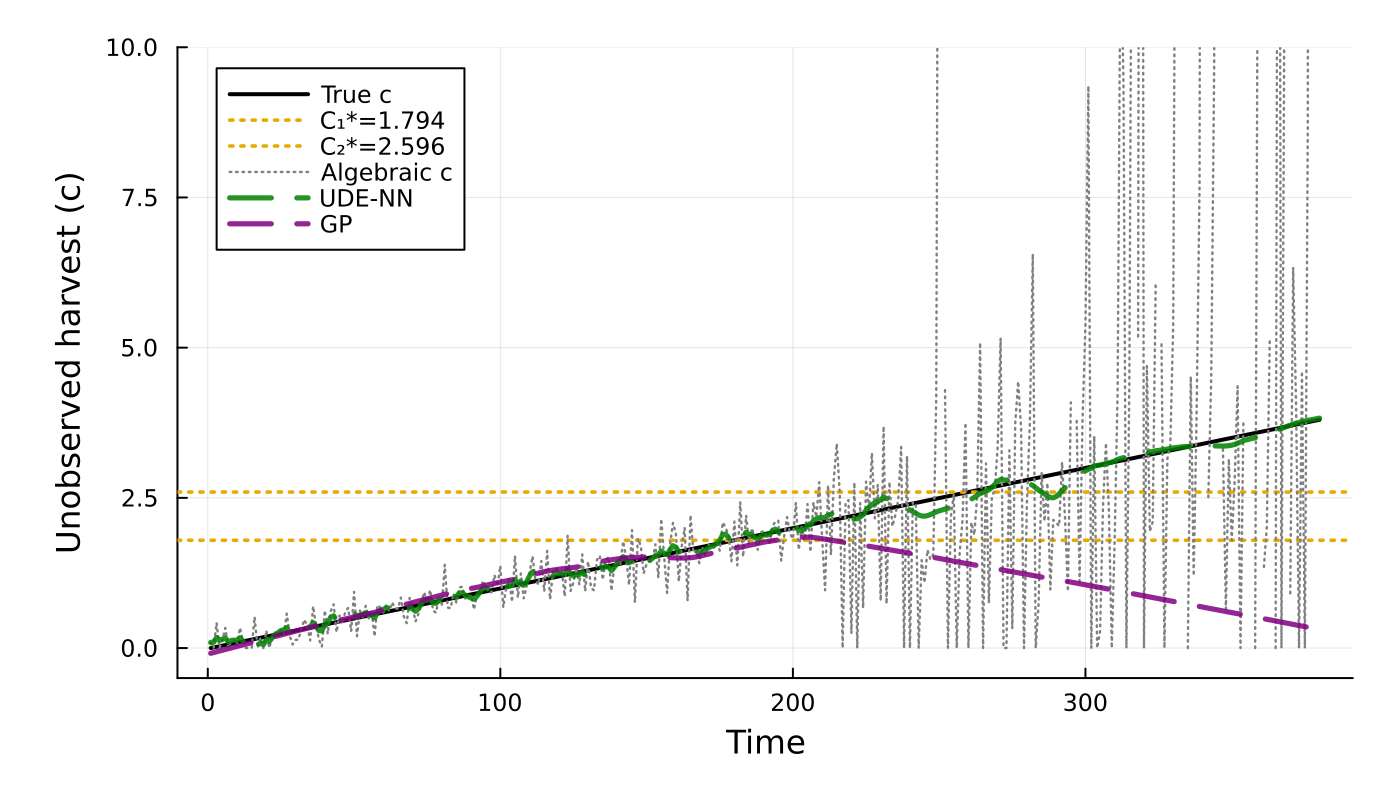
\includegraphics[width=0.8\linewidth]{revised_plots/C_hat_train380_seed42.png}
    \caption{Identification of the unobserved parameter $c_t$ from one of the random experiments. The actual parameter values (black) are compared with estimates from two methods: DE-Gaussian process (purple), and UDE-NN (green) and algebraically calculated harvest rate (dotted gray).}
    \label{fig:c_hat}
\end{figure}
% 
As the statistical properties of data change in different regimes, we evaluated the prediction performance of the UDE-NN and DE-GP methods by training with different data sizes (N) across three different regimes (Fig. \ref{fig:c_box}).
In Regime I and II (Fig. \ref{fig:c_box}, N=70, N=220), the DE-GP and UDE-NN approach achieved significantly lower RMSE values, than algebraically calculated $c_t$ demonstrating effective learning with limited data, similar to what we observed in Fig.\ref{fig:c_hat}, though DE-GP provides better estimates with relatively lower RMSE than UDE-NN, which can be attributed to the smooth approximation by DE-GP. However, in Regime III (Fig. \ref{fig:c_box}, N=300) UDE-NN outperforms DE-GP and alegbric method highlighting the effectiveness of neural networks in predicting unobserved bifurcation parameter.
% 
% 
\begin{figure}
    \centering
    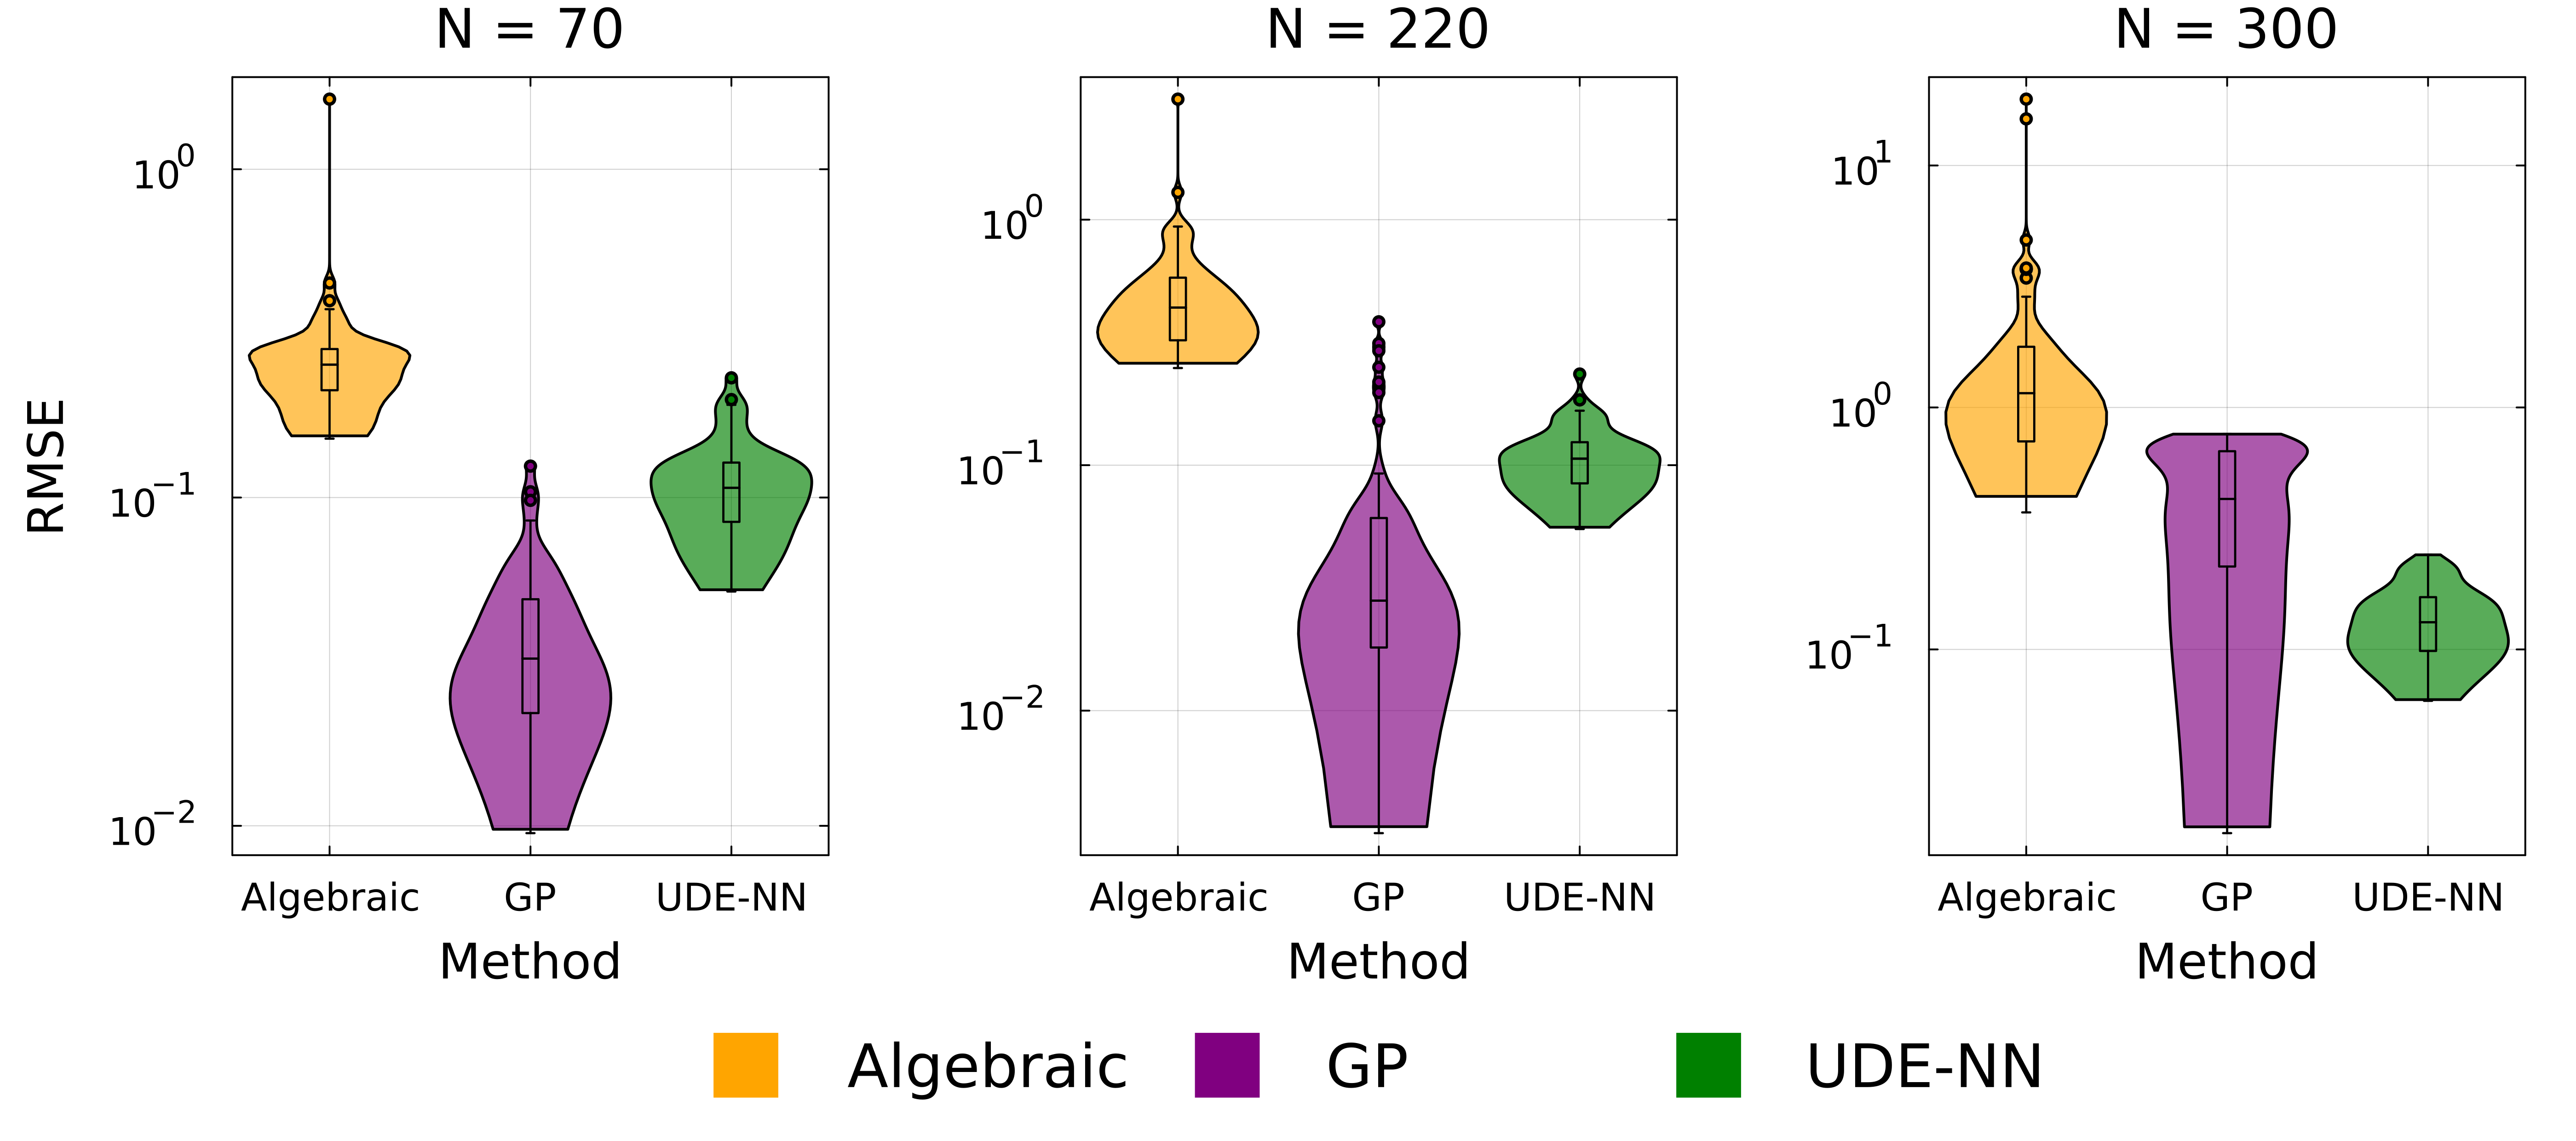
\includegraphics[width=\linewidth]{revised_plots/violin_rmseC.png}
    \caption{Violin-boxplots of root mean square error (RMSE) values for the predicted unobserved parameter $\hat{c}_t$ across different regimes over 50 random experiments. Results are given for high abundance regime I (N=70), intermediate flickering regime II (N=220), and low abundance regime III (N=300). The bottom and top of each box represent the first and third quartiles, respectively. The horizontal line inside the box indicates the median. Whiskers extend to the smallest and largest values within 1.5 times the interquartile range, and points beyond the whiskers represent outliers. The green boxes represent the universal dynamic equation with a neural network (UDE-NN), the purple boxes and yellow boxes represent error distributions for DE-Gaussian process (GP) and algebrically calculated harvest rates.}
    \label{fig:c_box}
\end{figure}
% 
% 
% In the classification context, the highest values of the F-score indicated that UDE-NN outperforms the DE-GP approximation technique in identifying the correct regime influenced by unobserved parameters (harvest rates) in the system (Fig. \ref{fig:fscore}). This consistent prediction ability across different regimes highlights the robustness of UDE-NN in accurately identifying critical transitions and making reliable predictions, even in complex and noisy environments. 
% 
In the classification context, the highest values of the F-score indicated that UDE-NN outperforms the DE-GP in identifying the correct regime influenced by unobserved parameters in the system (Fig. \ref{fig:fscore}). This consistent performance across regimes demonstrates that UDE-NN reliably identifies critical transitions and produces accurate predictions under noisy observations in single-species harvesting systems.
% 
\begin{figure}
    \centering
    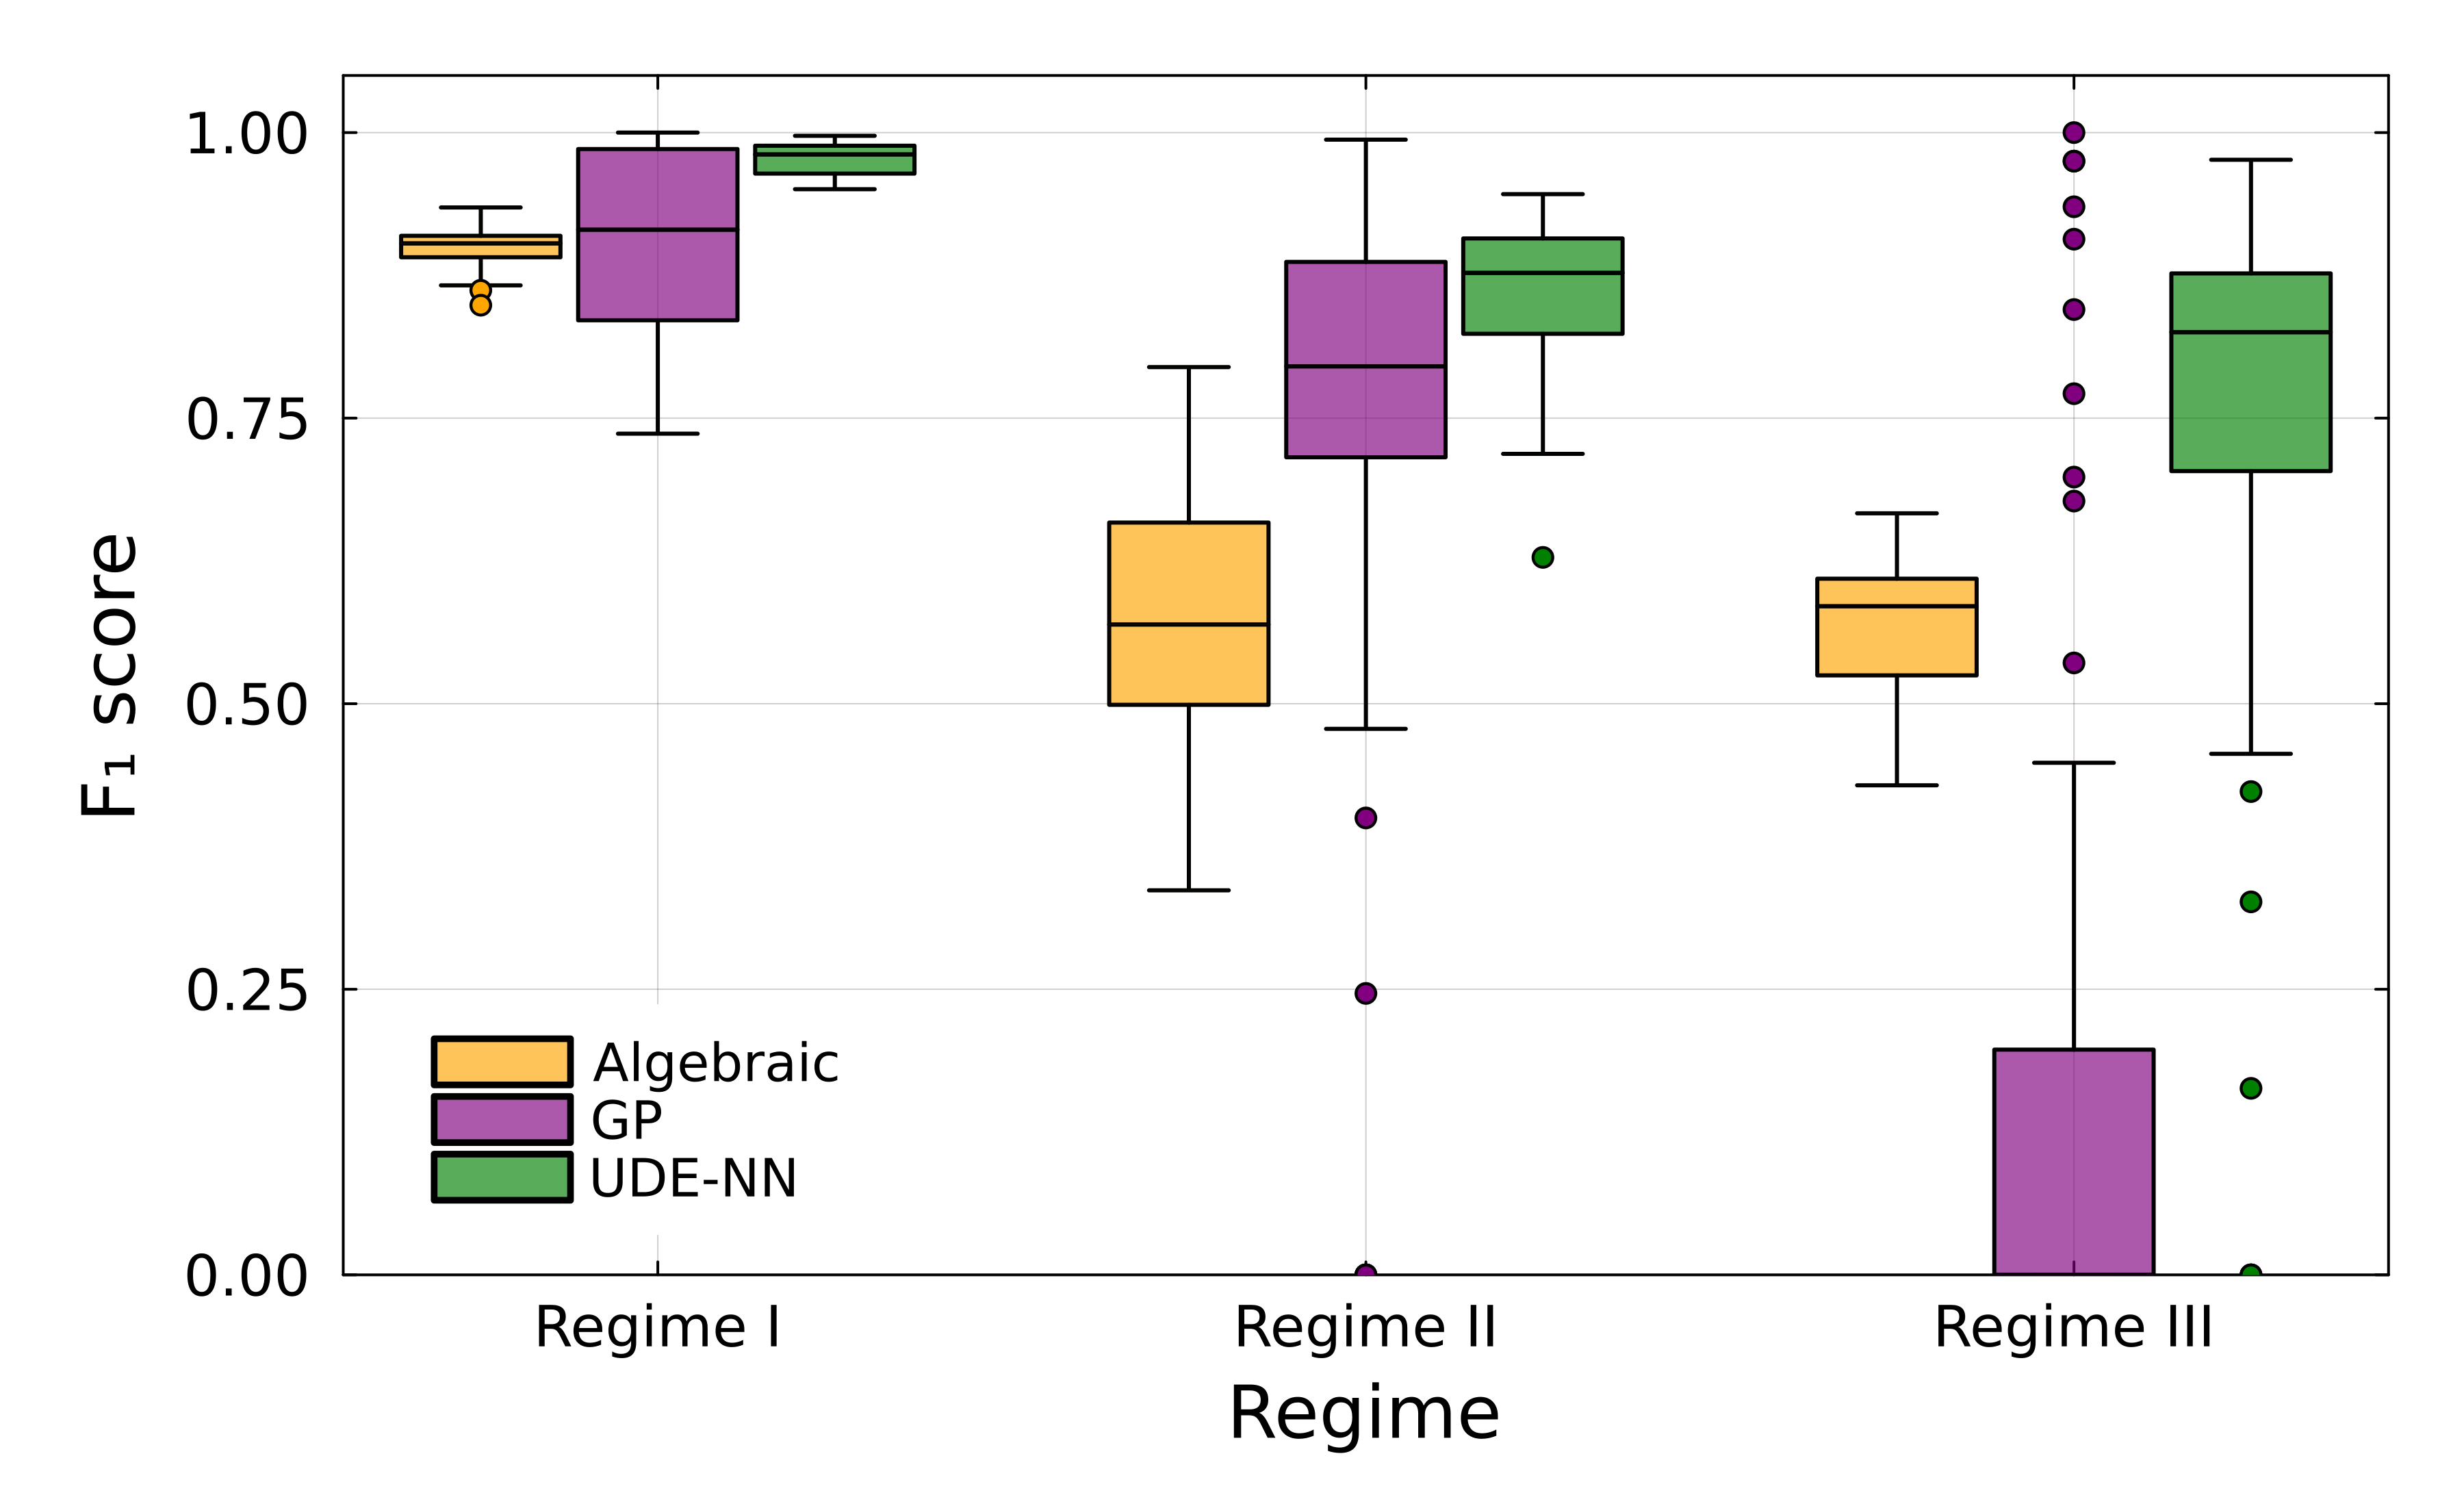
\includegraphics[width=0.8\linewidth]{revised_plots/box_f1_regimes.png}
    \caption{Classification-based predictions for the unobserved parameter $\hat{c_t}$, identifying the current categorical regime of the system (I, II, III) based on the predicted values. Boxplot shows F-score performance ranges (the higher, the better) in different regimes. Box color indicates methods, Algebric in yellow, DE-Gaussian process (GP) in purple, and our method, UDE-NN in green.}
    \label{fig:fscore}
\end{figure}
% 
However, the distribution of F-scores varies substantially between ecological regimes, reflecting differences in classification ability under changing system dynamics (Fig. \ref{fig:fscore}). In regime I (high abundance), the F-scores are tightly clustered, with the first quartile exceeding 0.75 and the upper whiskers approaching 1.0, indicating consistently high precision and recall. Regime II (flickering/bistable) exhibits moderate dispersion, with the first quartile around 0.75 and the highest values still reaching 1.0, suggesting reasonable classification confidence despite transient dynamics. In regime III (low abundance), the median F-score from UDE-NN remains relatively high ($\sim0.75$), but the DE-GP performance drops, indicating higher misclassification post transition. This regime-dependent spread in F-score distributions underscores the challenge of making reliable predictions under nonlinear transitions and ecological degradation.
% 
% 
\begin{figure}
    \centering
    
\includegraphics[width=0.99\textwidth]{revised_plots/x_rmsebox.png}
    \caption{Comparative forecast performance using the root mean square error (RMSE) metric across different regimes and forecast horizons. Blue, yellow, olive and purple boxes represent ARIMA, RandomWalk, LSTM, and DE-Gaussian process methods, respectively, and green boxes correspond to the UDE-NN method. Grouped boxplots of the performance metric after training on 70 data points (Regime I), 220 data points (Regime II), and 300 data points (Regime III).}
    \label{fig:rmse_forecasts_box}
\end{figure}
% 
% 
% ============================================
\subsection{Near-Term Forecasts of Regime Shifts}
% ============================================
% We used trained models to forecast changes in population abundances as a function of different harvest rates. Figure \ref{fig:forecast1x3}. illustrates the predicted abundances, and the different colored lines corresponding to different harvest rate scenarios. The results highlight the potential for recovery of the system with lower harvest rates [figure \ref{fig:forecast1x3}. Panel D.] regardless of the current regime. It also highlights that adopting lower harvest rates can prevent irreversible collapse and enable recovery, whereas higher harvest rates drive the system toward the unstable regime II or the low-abundance regime III. 

% Figure \ref{fig:forecast} shows the comparisons of the forecast uncertainty between different methods. The UDE-NN model, with an embedded neural network, demonstrates a narrower confidence interval, indicating reduced uncertainty in forecasting. In contrast, other DE methods exhibit increasing uncertainty as the forecast horizon is extended. Additionally, the results suggest that the algorithms had more uncertainty in Regime II, which is the system's flickering regime.
% 
The forecast performance of the implemented approaches was evaluated for varying horizons (time-steps) \{1, 5, 10, 15\} using the RMSE metric (Fig. \ref{fig:rmse_forecasts_box}). 
Methods using known dynamics (UDE-NN and DE-GP) consistently showed competetive performance for one-step-ahead forecast (horizon = 1) and slightly improved performance with lower median RMSE values for the forecast horizon of 5 time-steps (Fig. \ref{fig:rmse_forecasts_box}, N=220). Both methods showed relatively better performance than the alternative methods in the flickering regime II (Table \ref{tab:forecast_table}, N70, N=220).
Mann-Whitney U-test shows significant differences ($p<1e-8$) in RMSE performance between methods that use known dynamics (UDE-NN and DE-GP) and those without known dynamics (ARIMA, Random-Walk, LSTM) for one-step forecasts under regime I and II (N=70, N=220).
Forecast ability of all the methods degrade relatively with the increase in horizon length, which was expected given the highly stochastic nature of this system.
% 
In regime-III forecast UDE-NN method outperforms alternative methods for longer horizon, while performance of DE-GP method declines heavily with increasinging horizon length (Table \ref{tab:forecast_table}, N=300). Overall, the experiment suggested that UDE-NN method using known dynamics provides more promising short-term forecasting capabilities, and have potential for improvement in long-term forecasting capabilities.
%  
% 
% The Mann-Whitney U test did not show significant differences in RMSE performance between the DE-GP and the UDE-NN method for state forecasting (p = 0.528). The balanced rank sums (2617.0 vs 2433.0) and small effect size (0.0163) suggest that DE-GP and UDE-NN methods achieve similar levels of forecasting accuracy for state variables.

% The uncertainty analysis reveals distinct performance characteristics across different regimes. Dataset 530 presents moderate complexity where most methods exhibit considerable prediction uncertainty, yet UDE-NN maintains consistently low uncertainty, demonstrating superior ability to capture underlying dynamics without being overly sensitive to noise in this intermediate-flickering regime.

% Dataset 800 represents a qualitatively different, low-variance stable regime where all methods achieve significantly lower RMSE values with substantially reduced variance. UDE-NN particularly benefits from this stability, achieving remarkably tight performance with RMSE values consistently below 0.1 and minimal variance across all forecasting horizons. This progression demonstrates that UDE-NN not only outperforms competing methods but also exhibits superior scalability, becoming increasingly stable and accurate as more data becomes available to characterize the system's true dynamics.


% \begin{table*}
%     \centering
%     \caption{Quantitative comparison of forecasts using root mean square error (RMSE). Median RMSE values are reported across different training scenarios based on the number of training data points, approximation techniques within the difference equation (DE) and universal dynamic equation (UDE) frameworks, and forecast horizons (1, 5, 10, or 15 time steps). The lowest RMSE values per training set are in bold.}
%     \begin{tabular}{|c|l|c|c|c|c|c|}
%     \hline
%     \parbox{3cm}{Training datasize (N)} & Method & RMSE-1 & RMSE-5 & RMSE-10 & RMSE-15 & \parbox{3.2cm}{Mean training time (s)}\\ \hline
        
%         204 & ARIMA & 0.5234 & 0.9572 & 1.1842 & 1.4818 & 17.21 \\ 
%         204 & RandomWalk & 0.5063 & 0.9003 & \textbf{1.1733} & \textbf{1.4685} & 1.05 \\ 
%         204 & LSTM & 0.7487 & 1.1642 & 1.6540 & 2.2764 & 58.05 \\ 
%         204 & GP & \textbf{0.1760} & \textbf{0.7787} & 1.3053 & 1.6314 & 533.11 \\ 
%         204 & UDE & \textbf{0.1760} & 0.7886 & 1.2447 & 1.4871 & 246.34 \\ \hline
        
%         530 & ARIMA & 0.3093 & 0.673 & 0.7556 & 0.7862 & 19.52 \\ 
%         530 & RandomWalk & 0.3257 & 0.6564 & 0.7743 & 0.7918 & 1.13 \\
%         530 & LSTM & 0.4090 & 1.0727 & 1.3187 & 1.6924 & 327.31 \\ 
%         530 & GP & \textbf{0.1938} & \textbf{0.3799} & \textbf{0.3965} & \textbf{0.5121} & 3769.40 \\ 
%         530 & UDE & \textbf{0.1938} & 0.3883 & 0.424 & 0.5269 & 617.21 \\ \hline
        
%         800 & ARIMA & 0.1986 & 0.2903 & 0.2859 & 0.2968 & 20.73 \\ 
%         800 & RandomWalk & 0.1982 & 0.2923 & 0.2941 & 0.2985 & 1.14 \\
%         800 & LSTM & 0.1856 & 0.2541 & 0.2534 & 0.2614 & 785.05 \\ 
%         800 & GP & \textbf{0.1405} & 0.2495 & 0.2442 & 0.2413 & 9330.91 \\ 
%         800 & UDE & \textbf{0.1405} & \textbf{0.2451} & \textbf{0.2383} & \textbf{0.2353} & 904.33 \\ \hline
%     \end{tabular}
%     \label{tab:forecast_table}
% \end{table*}
% 
% 
% 
\begin{table}
\centering
\caption{Quantitative comparison of forecasts using root mean square error (RMSE). Median RMSE values are reported across different training scenarios based on the number of training data points, approximation techniques within the difference equation (DE) and universal dynamic equation (UDE) frameworks, and forecast horizons (1, 5, 10, or 15 time steps). The lowest RMSE values per training set are in bold.}
\label{tab:forecast_table}
\begin{tabular}{l l >{$}c<{$} >{$}c<{$} >{$}c<{$} >{$}c<{$} >{$}c<{$}}
\toprule
\textbf{N} & \textbf{Method} & \text{RMSE-1} & \text{RMSE-5} & \text{RMSE-10} & \text{RMSE-15} & \text{Training Time} \\ 
\midrule
70  & ARIMA  & 0.719 \pm 0.559 & 1.139 \pm 0.733 & 1.650 \pm 0.839 & 2.049 \pm 0.955 & 18.6 \pm 0.8 \\
    & RW     & 0.727 \pm 0.573 & 1.164 \pm 0.668 & 1.635 \pm 0.788 & 1.918 \pm 0.985 & 1.2 \pm 0.2 \\
    & LSTM   & 1.654 \pm 1.391 & 2.251 \pm 1.511 & 2.710 \pm 1.542 & 3.074 \pm 1.580 & 44.8 \pm 2.4 \\
    & UDE-NN & 0.297 \pm 0.321 & 0.800 \pm 0.438 & 1.245 \pm 0.554 & 1.514 \pm 0.693 & 101.3 \pm 4.1 \\
    & DE-GP     & \mathbf{0.271 \pm 0.274} & \mathbf{0.747 \pm 0.395} & \mathbf{1.190 \pm 0.519} & \mathbf{1.473 \pm 0.671} & 216.1 \pm 5.1 \\ 
\addlinespace
220 & ARIMA  & 0.532 \pm 0.516 & 1.024 \pm 0.852 & 1.475 \pm 1.534 & 1.695 \pm 1.860 & 20.1 \pm 1.0 \\
    & RW     & 0.510 \pm 0.492 & 0.981 \pm 0.801 & 1.433 \pm 1.474 & 1.641 \pm 1.803 & 1.2 \pm 0.2 \\
    & LSTM   & 1.449 \pm 1.634 & 2.480 \pm 2.348 & 3.235 \pm 2.769 & 3.675 \pm 2.966 & 57.8 \pm 5.1 \\
    & UDE-NN & 0.295 \pm 0.241 & \mathbf{0.630 \pm 0.499} & \mathbf{1.134 \pm 1.361} & \mathbf{1.344 \pm 1.782} & 158.9 \pm 5.8 \\
    & DE-GP     & \mathbf{0.263 \pm 0.219} & 0.662 \pm 0.480 & 1.272 \pm 1.352 & 1.613 \pm 1.880 & 761.3 \pm 19.3 \\ 
\addlinespace
300 & ARIMA  & 0.293 \pm 0.251 & 0.371 \pm 0.341 & 0.571 \pm 0.822 & 0.760 \pm 1.498 & 20.3 \pm 1.2 \\
    & RW     & 0.311 \pm 0.285 & \mathbf{0.340 \pm 0.197} & \mathbf{0.492 \pm 0.646} & 0.629 \pm 1.289 & 1.2 \pm 0.1 \\
    & LSTM   & 0.592 \pm 0.980 & 1.081 \pm 1.737 & 1.596 \pm 2.406 & 1.953 \pm 2.858 & 492.0 \pm 150.7 \\
    & UDE-NN & \mathbf{0.239 \pm 0.208} & 0.383 \pm 0.598 & 0.502 \pm 1.026 & \mathbf{0.540 \pm 1.043} & 204.0 \pm 12.3 \\
    & DE-GP     & 0.339 \pm 0.316 & 1.110 \pm 1.698 & 2.019 \pm 2.623 & 2.569 \pm 2.936 & 1279.0 \pm 25.5 \\ 
\bottomrule
\end{tabular}
\end{table}
% 
% 
% ============================================
\subsection{Performance based on System Observability}
% ============================================
Table~\ref{tab:partially_obs}. summarizes latent parameter recovery and forecasting performance for UDE-NN and DE-GP across the two observability settings introduced in  Section~\ref{sec:obs_variants} --- fully observed ($x$, $i$) and partially observed ($x$ only). In both observation scenarios, UDE-NN substantially outperformed DE-GP on latent harvesting rate recovery: RMSE-C dropped from $1.017$ to $0.228$ in the fully observed case, and from $1.305$ to $1.110$ in the partially observed case, with a corresponding improvement in Macro-F1 from $0.501$ to $0.894$ and from $0.225$ to $0.613$ respectively.
UDE-NN reduced the error in harvesting rate recovery by a factor of roughly $35\times$ relative to the algebraic reference in the fully observed setting (RMSE-C $0.228$ vs.\ $8.111$), and by nearly $9\times$ in the partially observed setting (RMSE-C $1.110$ vs.\ $9.779$), demonstrating that jointly optimizing the latent trajectory and network weights yields substantially more reliable recovery than algebraic inversion alone. Forecasting accuracy, measured by RMSE at horizons 1 through 15, remained comparable between the two UDE-NN variants, suggesting that the additional difficulty of the partially observed setting penalizes latent recovery more than short-horizon abundance prediction. DE-GP forecast error grew substantially with horizon in both settings,
indicating that its latent $c_t$ estimates do not generalize well
beyond the training window under increasing harvesting pressure. Finally, UDE-NN was consistently faster to train than DE-GP by a factor of roughly $7$--$8\times$, a practical advantage in high-volume simulation studies.
% 
% 
\begin{table}[ht]
\centering
\caption{Performance comparison under different level of system knowledge i.e fully or partially observed system}
\label{tab:partially_obs}
\small
\begin{tabular}{l cccc}
\toprule
% \textbf{Term} & \multicolumn{4}{c}{\textbf{Holling3}} \\
% \midrule
\textbf{Type} & \multicolumn{2}{c}{\textbf{Fully Observed (x, i)}} & \multicolumn{2}{c}{\textbf{Partially Observed (x)}} \\
\cmidrule(lr){2-3} \cmidrule(lr){4-5}
\textbf{method} & \textbf{UDE-NN} & \textbf{DE-GP} & \textbf{UDE-NN} & \textbf{DE-GP} \\
\midrule
Training-Time & 260.1 $\pm$ 15.80 & 1872.5 $\pm$ 43.20 & 331.6 $\pm$ 11.60 & 2761.2 $\pm$ 62.80 \\
RMSE-C-alg & 8.111 $\pm$ 17.39 & 8.111 $\pm$ 17.39 & 9.779 $\pm$ 21.67 & 9.779 $\pm$ 21.67 \\
RMSE-C & \textbf{0.228 $\pm$ 0.10} & 1.017 $\pm$ 0.28 & \textbf{1.110 $\pm$ 0.65} & 1.305 $\pm$ 0.14 \\
Macro-F1 & \textbf{0.894 $\pm$ 0.08} & 0.501 $\pm$ 0.16 & \textbf{0.613 $\pm$ 0.14} & 0.225 $\pm$ 0.04 \\
RMSE-1 & 0.202 $\pm$ 0.15 & 0.365 $\pm$ 0.31 & 0.219 $\pm$ 0.15 & 0.362 $\pm$ 0.30 \\
RMSE-5 & 0.237 $\pm$ 0.10 & 1.271 $\pm$ 1.35 & 0.242 $\pm$ 0.10 & 0.970 $\pm$ 0.79 \\
RMSE-10 & 0.241 $\pm$ 0.08 & 3.287 $\pm$ 2.78 & 0.245 $\pm$ 0.08 & 2.657 $\pm$ 2.07 \\
RMSE-15 & 0.244 $\pm$ 0.08 & 4.469 $\pm$ 3.11 & 0.248 $\pm$ 0.08 & 3.678 $\pm$ 2.60 \\
\bottomrule
\end{tabular}
\end{table}
% 
% 
% 
% 
%%%%%%%%%%%%%%%%%%%%%%%%%%%%%%%%%%%%%%%%%%%%%
\section{Discussion}
\label{discussion}
%%%%%%%%%%%%%%%%%%%%%%%%%%%%%%%%%%%%%%%%%%%%%
% brief outcomes of our approach
Predicting regime shifts in systems where there are unobserved drivers remains a significant challenge in many domains \cite{dakos2015resilience, hamilton1989new, RegimeSwitching}. Our study demonstrates that UDEs (both based on neural networks and Gaussian processes) can effectively predict unobserved driving parameters in social-environmental systems experiencing regime shifts. The framework successfully estimated unobserved harvest rates from simulated abundance data alone while incorporating governing equations, achieving three key outcomes: 1) more accurate predictions of unobserved parameter changes (indicated by lower RMSE values), 2) successful regime identification based on predicted parameters (with high F-scores), and 3) competitive short-term forecasting performance compared to alternative approaches.
% 
The UDE method excels when systems exhibit explicit environmental stochasticity, where random fluctuations and unreported external forces create challenges for traditional forecasting approaches. By incorporating known mechanistic dynamics, UDEs can distinguish between stochastic noise and meaningful signals, enabling more reliable predictions even with noisy observations.
The approach is particularly powerful when systems contain unknown or unreported influencing parameters that are difficult to estimate through direct observation. These unobserved drivers can emerge from multiple sources: technological and measurement limitations including sensor failures and analytical methodology constraints \cite{rocke_modeling_2003, decorte_missing_2024}, microclimate heterogeneity creating fine-scale environmental variations that influence species interactions \cite{mislan_microclimate_2008}, temporal scale mismatches where ecological processes operate over different timescales than monitoring programs \cite{winkler_mismatches_2021}, subsurface processes that remain largely unobservable \cite{condon2021global}, legacy effects from historical disturbances that continue to influence contemporary ecosystem dynamics \cite{krause2020legacy}, economic and logistical constraints that limit monitoring coverage \cite{sparrow_effective_2020}, and cryptic ecological processes such as undiscovered species interactions \cite{bickford_cryptic_2007, uusitalo_hidden_2018}. These unobserved drivers can also emerge from illegal activities such as unreported fishing events, poaching, or other clandestine resource extraction activities that are deliberately concealed from monitoring systems. Crucially, when such hidden parameters significantly influence system regime transitions, UDEs can capture these effects within a mechanistic framework that maintains biological and physical realism.

The incorporation of known dynamics provides several advantages over purely data-driven approaches. Combining mechanistic models with data-driven approaches offers a powerful means of addressing regime shift predictions in dynamical systems. These mechanistic constraints help the neural network components learn system behavior faster and produce more reliable results by constraining the solution space to physically plausible outcomes. Furthermore, incorporating established ecological or physical principles enhances the interpretability of the model, allowing researchers and managers to understand not only what the model predicts, but also why those predictions make sense within known theoretical frameworks.

% Motivation from and advantages over existing methods?
Our UDE approach builds on and extends the valuable foundations established by current methods for predicting unobserved parameters in complex systems. Empirical dynamic modeling \cite{Munch2024} and statistical approaches have demonstrated significant success in identifying patterns in observed data and have been instrumental in advancing our understanding of complex system dynamics. Similarly, existing modeling approaches   \cite{Agan_etal,FERREGUETTI2018133} to estimating unobserved harvest or poaching rates have made important contributions to conservation science.

% Knowledge-based systems such as PoachNet \cite{hamed2024poachnet} pioneered the integration of domain expertise with predictive modeling, while data-driven geographical models \textcite{guru_etal} and game-theoretic frameworks such as CAPTURE \cite{nguyen2016capture} have advanced, sophisticated approaches to patrol planning under uncertainty \textcite{StayAhead}. 

Sparse system identification methods such as SINDy \cite{brunton2016discovering} and non-parametric approaches including Gaussian process methods \cite{alvarez2012kernels} have contributed valuable techniques to infer system dynamics from limited observations. In parallel, scientific machine learning approaches have developed distinct paradigms for discovering and modeling unobserved dynamics in complex systems. Physics-informed neural networks (PINNs) have demonstrated success in incorporating known physical laws while learning unknown parameters from sparse data \cite{raissi2019physics,karniadakis2021physics}. Neural ordinary differential equations (NODEs) \cite{chen2018neural} provide powerful frameworks for learning continuous-time dynamics directly from observations, while universal differential equation approaches \cite{rackauckas2020universal} have shown promise in combining mechanistic knowledge with machine learning for scientific discovery. These methods have proven particularly effective either when the underlying system structure is well-characterized or when sufficient data are available to learn complex mappings.

However, these approaches face inherent challenges when dealing with systems in which unobserved driving parameters exhibit their own complex temporal dynamics. While traditional methods excel at pattern recognition and strategic optimization, they typically rely on sparse and potentially biased observation data, making it difficult to model the dynamic adversarial behaviors that characterize many social-environmental systems. Our UDE framework complements these existing approaches by explicitly modeling and predicting the temporal evolution of hidden drivers within a mechanistic context, offering a distinct methodological contribution that addresses scenarios where traditional approaches may be limited.

Recent advances in reservoir computing for extracting slowly time-varying parameters \cite{tokuda2024prediction} and learning governing equations of unobserved states \cite{grigorian2025learning} have demonstrated the feasibility of inferring hidden dynamics from time series data. Our UDE framework extends these contributions through three key advances: 1) explicit incorporation of unobserved parameters within mechanistic model structures, 2) direct integration of known mechanistic dynamics into the fast dynamics model, and 3) application to regime-shifting systems between stable equilibrium points. The latter is a more challenging inference problem than the chaotic dynamics typically studied, as stable phases provide fewer informative signals about underlying parameter changes.

The broader Scientific Machine Learning landscape has seen significant advances through symbolic regression \cite{angelis2023artificial}, physics-informed neural networks (PINNs) \cite{cuomo2022scientific}, and Gaussian process-based modeling \cite{girard2005gaussian}. Our UDE framework builds on these innovations while specifically targeting the challenge of predicting the temporal evolution of unobserved driving forces. The neural network approximators within UDEs leverage the universal approximation capabilities demonstrated by these previous works, extending their application to high-dimensional systems with multiple interacting variables where complex nonlinear relationships between observed and unobserved components can be captured within mechanistic frameworks.

% limitations and future scope?
Despite its effectiveness, the UDE approach faces limitations that define the boundaries of its application and highlight areas for future development. The method relies heavily on a deep understanding of process-based or mechanistic models, which may not always be readily available for complex systems. Researchers must have sufficient knowledge of the dynamics of the underlying system to specify appropriate governing equations, which limits applicability in domains where the mechanistic understanding remains incomplete. The approach also requires robust approximation techniques to effectively capture the intricacies of the nonlinear or chaotic dynamics characteristic of ecological and stochastic systems \cite{jack_statespace}. Careful handling of feedback mechanisms proves crucial for accurate modeling, as mismanagement of these interactions can lead to erroneous conclusions or unstable model behavior. Current computational limitations become particularly pronounced when scaling to high-dimensional datasets with hundreds of interacting components, where complexity and computational demands increase significantly.

While our results show that UDEs do not consistently outperform alternative approaches in short-term forecast accuracy, this finding aligns with recent insights on the limitations of forecast-skill-based model selection. \textcite{boettiger2022forecast} demonstrates that selecting models based solely on forecast accuracy can create a `forecast trap', where seemingly superior statistical performance leads to worse real-world management outcomes. This occurs because forecast accuracy alone fails to capture the non-uniqueness of models and their differential impacts on management objectives. Our UDE framework addresses this challenge by prioritizing mechanistic understanding and parameter interpretability over pure forecast performance. By explicitly modeling unobserved driving parameters within established ecological frameworks, UDEs provide actionable insights into the causal mechanisms underlying regime shifts, information that may be more valuable for management intervention than marginally-improved forecast accuracy. This approach aligns with recommendations to promote broader sets of models rather than selecting based on forecast skill alone, emphasizing the importance of mechanistic insight for robust decision-making in social-environmental systems.

Future research should prioritize improving long-term forecasting ability, particularly for systems with regime shifts or strong stochastic dynamics, where prediction accuracy typically degrades over extended time horizons. Developing more efficient algorithms, advanced neural network architectures, and high-performance computing strategies will be essential for scaling to complex real-world systems. Furthermore, incorporating uncertainty quantification methods would enhance the reliability of the framework and provide confidence limits for management decisions based on the mechanistic foundation that distinguishes UDEs from purely statistical approaches.

% Real worls applications
% The UDE approach holds significant promise for addressing pressing conservation and environmental management challenges. In wildlife conservation, the method could revolutionize anti-poaching efforts by providing accurate estimates of illegal harvesting rates from population monitoring data alone. This capability would enable wildlife managers to design more effective patrol strategies and resource allocation decisions based on predicted rather than merely observed poaching activity.

The UDE approach shows potential for addressing conservation challenges, though validation with real-world data would be needed. In wildlife conservation, the method could potentially improve population assessments by estimating illegal harvest rates from monitoring data. This capability might help wildlife managers better understand the true impact of poaching on population dynamics and assess the effectiveness of existing conservation interventions.

For broader ecosystem management, the framework offers pathways toward early warning systems for regime shift detection across multiple domains. The approach can be extended to predict regime shifts in other complex systems, including political transitions, Earth system dynamics, and epidemiological patterns. Political regime shifts, often driven by economic instability, social movements, or institutional breakdowns, exhibit nonlinear dynamics that could be captured using hybrid mechanistic data-driven models. Similarly, regime shifts in the Earth system such as those quantified in the planetary boundaries framework \cite{rockstrom2009safe, steffen2015planetary} and research on cascading tipping points \cite{rocha2018cascading}—highlight the interconnected nature of environmental thresholds. Furthermore, epidemiological applications \cite{brauer2019mathematical}, such as predicting the spread of infectious diseases, could benefit from this approach by integrating mechanistic models of disease transmission with real-time data assimilation.

However, realizing these applications requires several key advances. Scaling computational efficiency for high-dimensional systems remains critical for handling the complexity of real-world scenarios. Developing robust methods for uncertainty quantification would also provide essential confidence measures for management decisions. 

% Furthermore, creating frameworks for integrating multiple data sources and handling incomplete or biased observational data would enhance practical applicability across diverse contexts.

% Conclusion
This work provides a new method for quantifying hidden dynamics in complex systems by directly predicting changes in unobserved parameters that drive regime shifts. This capability provides actionable information for management interventions and would be of great potential use for effective governance of social-ecological systems. The ability to predict not only what will happen but also the causal mechanisms of change can mean the difference between proactive management and reactive crisis response. As global systems face unprecedented pressures and regime shifts become increasingly common, tools that can peer into hidden mechanisms of change offer hope for more effective stewardship of social-ecological systems. The UDE framework has the potential to provide policy makers and resource managers with improved capabilities to design optimal control strategies. Future efforts could focus on scaling these methods to high-dimensional systems and validating their performance across diverse real-world applications. Ultimately, through new methods like SciML, we can improve our ability to predict and prepare for critical transitions in complex systems.



%%%%%%%%%%%%%%%%%%%%%%%%%%%%%%%%%%%%%%%%%%%%%
% \end{multicols}



% ========================================
\newpage
\section*{Appendix}
\appendix
\section{Mechanistic Model Parameters and Data Pre-Processing}

We simulated the \textcite{Tilman2024} model to generate time series data with different random seeds, by solving the discrete state-space equation \eqref{eq:discrete_time_x}. We considered the harvest rate as an unobserved parameter that monotonically increases between the suggested range [0,4] in \textcite{Tilman2024}. This process provides time-series observations $\hat{x}, \hat{i}$ corresponding to the environmental state and the term of noise in the system.
The parameter values are listed in table \ref{tab:def_params}.

\begin{table}[H]
    % \centering
    \caption{\textcite{Tilman2024} mechanistic model parameters}
    \begin{tabular}{l|l|l}
    \hline
        \textbf{Variable} & \textbf{Value} & \textbf{Description} \\ \hline
        $x_t$ & 0-20 & Current environmental state ($x_0$ = 10.0) \\ 
        $i_t$ &  & Auto-correlated red noise \\ 
        $T$ & 30 & Timescale over which noise becomes uncorrelated \\ 
        $\eta_t$ & 0 & i.i.d. normal error term \\ 
        $\beta$ & 0.07 & The standard deviation of $\eta$'s \\ 
        $r$ & 1 & Resource growth rate \\ 
        $K$ & 10 & Resource carrying capacity \\ 
        $c_t$ & .0-4.0 & harvest rate \\ 
        $h$ & 1 & harvest half-saturation constant \\ \hline
    \end{tabular}
    \label{tab:def_params}
\end{table}
% 
% 
% 
% 
% We used trained models to forecast changes in population abundances as a function of different harvest rates. Figure \ref{fig:forecast1x3} illustrates the predicted abundances, and the different colored lines corresponding to different harvest rate scenarios. The results highlight the potential for recovery of the system with lower harvest rates (Fig. \ref{fig:forecast1x3}D) regardless of the current regime. It also highlights that adopting lower harvest rates can prevent irreversible collapse and enable recovery, whereas higher harvest rates drive the system toward the unstable regime II or the low-abundance regime III. 



% \begin{figure*}[b]
%     \centering
%     \includegraphics[width=0.99\textwidth]{figures/forecast_2x3.png}
%     \caption{Forecasts of population abundances under different harvest rates $c$ in each regime. An example time series of a noisy environmental state $y_t$ simulated for 400 time steps (A). The dashed boxes show insets for regime I forecasts (B), regime II forecasts (C), and regime III forecasts (D) under increasing harvest rates.}
%     \label{fig:forecast1x3}
% \end{figure*}



% % =============================================
% % FOrecast figures
% \begin{figure*}
%     \centering
%     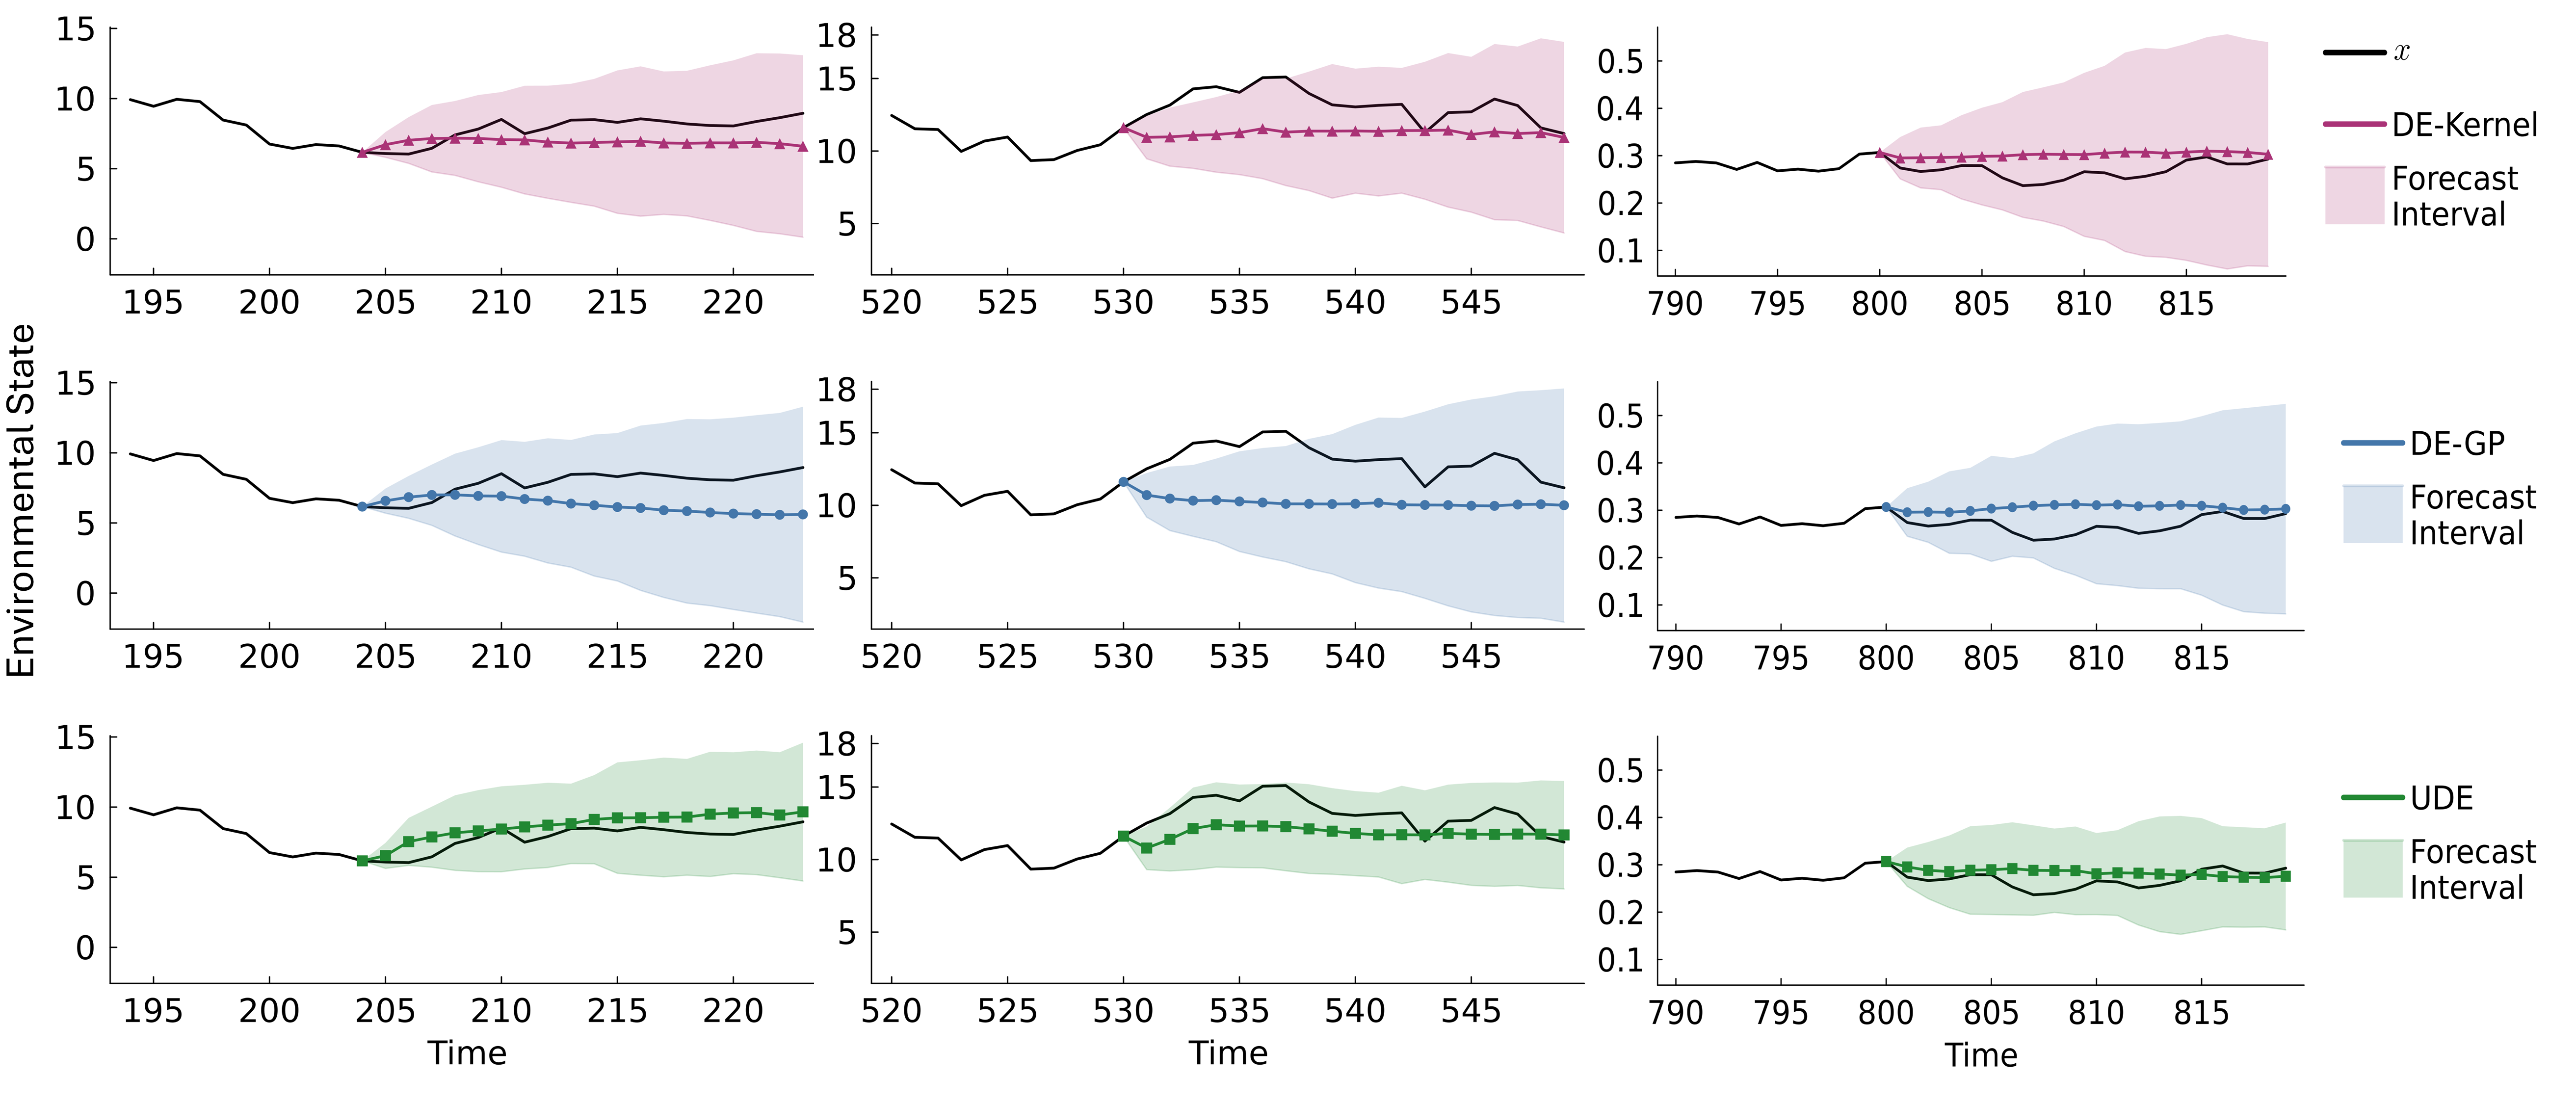
\includegraphics[width=0.99\textwidth]{figures/forecast_CI_3x3.png}
%     \caption{Forecasts and confidence intervals for the environmental state $x$ across different regimes using comparative methods. Column 1 displays predictions for regime I, column 2 for regime II, and column 3 for regime III. Average forecast values are represented as points and lines, with confidence intervals given as shaded regions. The methods are Kernel-based parameter approximation, Gaussian process (GP) augmentation, and universal dynamic equation (UDE). Note the different y-axis scales per column.}
%     \label{fig:forecast}
% \end{figure*}


% Figure \ref{fig:forecast} shows the comparisons of the forecast uncertainty between different methods. The UDE-NN model, with an embedded neural network, demonstrates a narrower confidence interval, indicating reduced uncertainty in forecasting. In contrast, other DE methods exhibit increasing uncertainty as the forecast horizon is extended. Additionally, the results suggest that the algorithms had more uncertainty in Regime II, which is the system's flickering regime.
% --------------
\section{Performance Evaluation Based on Data Availability}
% --------------
We also extended our experiments to evaluate how performance degrades under reduced data availability, summarized in Table~\ref{tab:sampled_data}, covering three sampling scenarios: fully observed ($N=380$), and two sparse observation scenarios subsampling every third ($N=126$) and every sixth ($N=63$) time step.

UDE-NN maintained strong latent recovery under moderate sparsity, with RMSE-C increasing only marginally from $0.228$ at full density to $0.314$ at $N=126$, and Macro-F1 remaining high at $0.843$, suggesting that the joint trajectory-network optimization is robust to a threefold reduction in observations. At the more aggressive sampling scenario ($N=63$), RMSE-C rose to $0.715$ and Macro-F1 dropped to $0.620$, indicating that reliable regime classification becomes more challenging when fewer than one-sixth of time steps are observed, though UDE-NN still outperformed DE-GP at this level ($0.715$ vs.\ $0.905$). DE-GP performance degraded more gradually on RMSE-C across sampling scenarios ($1.017 \to 1.070 \to 0.905$), but its forecast error at longer horizons remained consistently high, with RMSE-15 near $4.5$ in both the full and $N=126$ settings, converging toward UDE-NN only at the most aggressive sparsity where both methods face identifiability limits. 
% Training time for GP decreased substantially with sparser data ($1872 \to 917 \to 688$ seconds), while UDE-NN training time remained nearly constant across all three conditions, reflecting the fixed-architecture optimization that is largely insensitive to the number of observed points.
% 
\begin{table}[ht]
\centering
\caption{UDE Performance based on amount of observed training data under different data sampling conditions}
\label{tab:sampled_data}
\small
\setlength{\tabcolsep}{3pt}
\begin{tabularx}{\textwidth}{l @{\extracolsep{\fill}} cccccc}
\toprule
 & \multicolumn{2}{c}{\textbf{Full observed data}} & \multicolumn{2}{c}{\textbf{Sampled (N=126)}} & \multicolumn{2}{c}{\textbf{Sampled (N=63)}} \\
 & \multicolumn{2}{c}{\textbf{(N=380)}} & \multicolumn{2}{c}{\textbf{(freq=3)}} & \multicolumn{2}{c}{\textbf{(freq=6)}} \\
\cmidrule(lr){2-3} \cmidrule(lr){4-5} \cmidrule(lr){6-7}
\textbf{Method} & \textbf{UDE-NN} & \textbf{GP} & \textbf{UDE-NN} & \textbf{DE-GP} & \textbf{UDE-NN} & \textbf{DE-GP} \\
\midrule
RMSE-C-alg & $8.111 \pm 17.39$ & $8.111 \pm 17.39$ & $3.610 \pm 5.15$ & $3.610 \pm 5.15$ & $3.411 \pm 3.87$ & $3.411 \pm 3.87$ \\
RMSE-C & {$\mathbf{0.228 \pm 0.10}$} & $1.017 \pm 0.28$ & $\mathbf{0.314 \pm 0.17}$ & $1.070 \pm 0.30$ & $\mathbf{0.715 \pm 0.34}$ & $0.905 \pm 0.34$ \\
Macro-f1 & $\mathbf{0.894 \pm 0.08}$ & $0.501 \pm 0.16$ & $\mathbf{0.843 \pm 0.12}$ & $0.460 \pm 0.19$ & $\mathbf{0.620 \pm 0.19}$ & $0.505 \pm 0.22$ \\
RMSE-1 & $0.202 \pm 0.15$ & $0.365 \pm 0.31$ & $0.244 \pm 0.41$ & $0.295 \pm 0.27$ & $0.270 \pm 0.37$ & $0.259 \pm 0.23$ \\
RMSE-5 & $0.237 \pm 0.10$ & $1.271 \pm 1.35$ & $0.398 \pm 1.04$ & $1.425 \pm 1.41$ & $0.843 \pm 1.29$ & $0.876 \pm 0.96$ \\
RMSE-10 & $0.241 \pm 0.08$ & $3.287 \pm 2.78$ & $0.437 \pm 1.31$ & $3.456 \pm 2.99$ & $1.718 \pm 2.83$ & $2.273 \pm 2.54$ \\
RMSE-15 & $0.244 \pm 0.08$ & $4.469 \pm 3.11$ & $0.449 \pm 1.37$ & $4.486 \pm 3.30$ & $2.096 \pm 3.29$ & $3.219 \pm 3.04$ \\
\bottomrule
\end{tabularx}
\end{table}
% 
% 
% --------------
\section{Performance Evaluation Based on System's Knowledge}
% --------------
We further evaluated robustness to the assumed functional form of the consumption term by comparing UDE-NN and DE-GP performance across four harvesting specifications: Holling type-III ($x^2/(x^2+h^2)$), constant ($1$), linear ($x$), and quadratic ($x^2$), with results summarized in Table~\ref{tab:consumption_comparison}.

UDE-NN achieved its strongest latent recovery under the Holling type-III term (RMSE-C $0.228$, Macro-F1 $0.894$), which corresponds to the true generating model, confirming that correct functional specification yields the most accurate regime identification.
Under misspecified consumption terms, UDE-NN performance degraded but remained competitive: RMSE-C ranged from $0.978$ (quadratic) to $1.573$ (constant), with Macro-F1 highest under the quadratic term ($0.548$) and lowest under the linear term ($0.213$), where both methods effectively collapsed to near-random regime classification. DE-GP showed a similar pattern of degradation but with consistently higher RMSE-C and lower Macro-F1 than UDE-NN across all four terms, with the exception of the constant specification where both methods performed comparably ($1.573$ vs.\ $1.521$). Forecast accuracy followed a different ordering: the linear consumption term yielded the lowest forecast error for both methods (RMSE-15 of $0.068$ and $1.251$ respectively), likely because the simpler functional form produces smoother abundance trajectories that are easier to extrapolate, even when latent $c_t$ recovery is poor. Training time was broadly consistent across consumption terms for UDE-NN, while DE-GP showed higher variance under the constant specification, suggesting sensitivity of the kernel optimization to the shape of the latent trajectory.
\begin{table}[ht]
\centering
\caption{Comparison of UDE-NN and DE-GP performance across different Consumption Terms (known dynamics)  ; On Full timeseries ; Fully observed system with abundance and noise (x, i)}
\label{tab:consumption_comparison}
\small
\resizebox{\textwidth}{!}{%
\begin{tabular}{l cccccccc}
\toprule
\textbf{Term} & \multicolumn{2}{c}{\textbf{Holling-III ($x^2/(x^2+h^2)$)}} & \multicolumn{2}{c}{\textbf{Constant (1)}} & \multicolumn{2}{c}{\textbf{Linear (x)}} & \multicolumn{2}{c}{\textbf{Quadratic (x2)}} \\
\cmidrule(lr){2-3} \cmidrule(lr){4-5} \cmidrule(lr){6-7} \cmidrule(lr){8-9}
\textbf{method} & \textbf{UDE-NN} & \textbf{DE-GP} & \textbf{UDE-NN} & \textbf{DE-GP} & \textbf{UDE-NN} & \textbf{DE-GP} & \textbf{UDE-NN} & \textbf{DE-GP} \\
\midrule
Training-Time & 260.1 $\pm$ 15.89 & 1872.5 $\pm$ 43.24 & 206.8 $\pm$ 8.92 & 2137.3 $\pm$ 298.68 & 329.8 $\pm$ 12.72 & 1858.8 $\pm$ 39.56 & 333.5 $\pm$ 8.32 & 1873.1 $\pm$ 47.86 \\
RMSE-C-alg & 8.111 $\pm$ 17.39 & 8.111 $\pm$ 17.39 & 8.043 $\pm$ 17.21 & 8.043 $\pm$ 17.21 & 1.089 $\pm$ 0.09 & 1.089 $\pm$ 0.09 & 0.617 $\pm$ 0.27 & 0.617 $\pm$ 0.27 \\
RMSE-C & 0.228 $\pm$ 0.10 & 1.017 $\pm$ 0.28 & 1.573 $\pm$ 0.25 & 1.521 $\pm$ 0.33 & 1.262 $\pm$ 0.14 & 1.750 $\pm$ 0.03 & 0.978 $\pm$ 0.14 & 1.692 $\pm$ 0.02 \\
Macro-F1 & 0.894 $\pm$ 0.08 & 0.501 $\pm$ 0.16 & 0.440 $\pm$ 0.18 & 0.349 $\pm$ 0.17 & 0.213 $\pm$ 0.00 & 0.212 $\pm$ 0.00 & 0.548 $\pm$ 0.09 & 0.213 $\pm$ 0.00 \\
RMSE-1 & 0.202 $\pm$ 0.15 & 0.365 $\pm$ 0.31 & 0.339 $\pm$ 0.36 & 0.462 $\pm$ 0.39 & 0.039 $\pm$ 0.05 & 0.056 $\pm$ 0.06 & 0.169 $\pm$ 0.11 & 0.214 $\pm$ 0.14 \\
RMSE-5 & 0.237 $\pm$ 0.10 & 1.271 $\pm$ 1.35 & 0.951 $\pm$ 1.53 & 2.543 $\pm$ 2.27 & 0.052 $\pm$ 0.05 & 0.163 $\pm$ 0.26 & 0.415 $\pm$ 0.16 & 0.959 $\pm$ 0.45 \\
RMSE-10 & 0.241 $\pm$ 0.08 & 3.287 $\pm$ 2.78 & 1.730 $\pm$ 2.76 & 4.756 $\pm$ 3.42 & 0.061 $\pm$ 0.08 & 0.662 $\pm$ 1.09 & 0.492 $\pm$ 0.15 & 1.214 $\pm$ 0.42 \\
RMSE-15 & 0.244 $\pm$ 0.08 & 4.469 $\pm$ 3.11 & 2.081 $\pm$ 3.22 & 5.521 $\pm$ 3.72 & 0.068 $\pm$ 0.11 & 1.251 $\pm$ 1.65 & 0.516 $\pm$ 0.15 & 1.267 $\pm$ 0.39 \\
\bottomrule
\end{tabular}%
}
\end{table}



% --------------
\section{Performance Evaluation Based on Parameter Sensitivity}
% --------------
Latent harvesting pressure recovery under the same parameter misspecification scenarios is reported in Table~\ref{tab:params_c}, complementing the forecast results in Table~\ref{tab:params_x}.

Under the baseline configuration, UDE-NN achieved strong latent recovery (RMSE-C $0.228$, Macro-F1 $0.894$), substantially outperforming DE-GP (RMSE-C $1.017$, Macro-F1 $0.501$). Misspecifying $h=2.0$ caused a sharp deterioration in UDE-NN latent recovery (RMSE-C $3.349$), while DE-GP degraded more modestly (RMSE-C $1.332$); a larger half-saturation constant flattens the consumption response at low abundance, reducing the signal available to distinguish harvesting from growth, and making the joint trajectory optimization more sensitive to initialization. Treating $h$ as a learnable parameter within the UDE framework would be a natural direction to reduce this sensitivity.
% 
Under $K=20.0$, both methods struggled with regime classification (UDE-NN Macro-F1 $0.321$, DE-GP $0.102$), as the wider dynamic range of $x_t$ stretches the latent space in which $c_t$ must be recovered, effectively diluting the regime-relevant signal in flickering regime; incorporating $K$-normalized state representations or abundance-conditioned priors on $c_t$ could help constrained recovery in high-capacity systems. At high growth rate ($r=2.0$, $K=1.0$), UDE-NN and DE-GP showed poor performance (Macro-F1 $0.268$ vs.\ $0.272$), suggesting that when population dynamics are fast and occur over a narrow abundance range, the signatures of regime transitions become difficult to detect from noisy observations alone; denser sampling
or longer training windows may help in such settings.
% 
% 
\begin{table}[H]
\centering
\caption{UDE Model Performance Comparison}
\label{tab:params_c}
\begin{tabular}{llccc}
\hline
\textbf{UDE-Parameters} & \textbf{Method} & \textbf{RMSE-C-ALG} & \textbf{RMSE-C} & \textbf{Macro F1} \\ \hline
(r=1.0; K=10.0; h=1.0) & UDE-NN & $8.111 \pm 17.39$ & $0.228 \pm 0.10$ & $0.894 \pm 0.08$ \\
                      &DE-GP     & $8.111 \pm 17.39$ & $1.017 \pm 0.28$ & $0.501 \pm 0.16$ \\ \hline
(r=1.0; K=10.0; h=2.0) & UDE-NN & $33.421 \pm 69.47$ & $3.349 \pm 0.99$ & $0.765 \pm 0.13$ \\
                      &DE-GP     & $33.421 \pm 69.47$ & $1.332 \pm 0.30$ & $0.487 \pm 0.19$ \\ \hline
(r=1.0; K=20.0; h=1.0) & UDE-NN & $10.178 \pm 16.83$ & $4.057 \pm 1.23$ & $0.321 \pm 0.14$ \\
                      &DE-GP     & $10.178 \pm 16.83$ & $3.538 \pm 0.72$ & $0.102 \pm 0.07$ \\ \hline
(r=2.0; K=1.0; h=1.0) & UDE-NN & $13.605 \pm 28.10$ & $2.258 \pm 0.48$ & $0.268 \pm 0.12$ \\
                      &DE-GP     & $13.605 \pm 28.10$ & $1.683 \pm 0.23$ & $0.272 \pm 0.15$ \\ \hline
\end{tabular}
\end{table}
% 
% 
\begin{table}[H]
\centering
\caption{Predictive Performance Comparison (RMSE Over Forecast Horizons)}
\label{tab:params_x}
\small
\begin{tabular}{llcccc}
\hline
\textbf{UDE-Parameters} & \textbf{Method} & \textbf{RMSE-1} & \textbf{RMSE-5} & \textbf{RMSE-10} & \textbf{RMSE-15} \\ \hline
& ARIMA & $0.257 \pm 0.23$ & $0.294 \pm 0.15$ & $0.311 \pm 0.13$ & $0.312 \pm 0.13$ \\
& RW    & $0.273 \pm 0.21$ & $0.286 \pm 0.14$ & $0.302 \pm 0.12$ & $0.304 \pm 0.12$ \\
& LSTM  & $0.354 \pm 0.57$ & $0.461 \pm 0.85$ & $0.622 \pm 1.28$ & $0.799 \pm 1.66$ \\
(r=1.0; K=10.0; h=1.0) & UDE-NN & $0.202 \pm 0.15$ & $0.237 \pm 0.10$ & $0.241 \pm 0.08$ & $0.244 \pm 0.08$ \\
(r=1.0; K=10.0; h=1.0) & DE-GP     & $0.365 \pm 0.31$ & $1.271 \pm 1.35$ & $3.287 \pm 2.78$ & $4.469 \pm 3.11$ \\ \hline
& ARIMA & $0.256 \pm 0.23$ & $0.295 \pm 0.16$ & $0.313 \pm 0.13$ & $0.313 \pm 0.13$ \\
& RW    & $0.272 \pm 0.22$ & $0.287 \pm 0.15$ & $0.303 \pm 0.12$ & $0.304 \pm 0.12$ \\
& LSTM  & $0.358 \pm 0.58$ & $0.467 \pm 0.86$ & $0.632 \pm 1.30$ & $0.812 \pm 1.68$ \\
(r=1.0; K=10.0; h=2.0) & UDE-NN & $0.202 \pm 0.17$ & $0.244 \pm 0.11$ & $0.254 \pm 0.09$ & $0.255 \pm 0.09$ \\
(r=1.0; K=10.0; h=2.0) & DE-GP     & $0.459 \pm 0.43$ & $2.765 \pm 2.28$ & $5.524 \pm 3.17$ & $6.412 \pm 3.38$ \\ \hline
& ARIMA & $0.257 \pm 0.23$ & $0.294 \pm 0.15$ & $0.311 \pm 0.13$ & $0.312 \pm 0.13$ \\
& RW    & $0.273 \pm 0.21$ & $0.286 \pm 0.14$ & $0.302 \pm 0.12$ & $0.304 \pm 0.12$ \\
& LSTM  & $0.352 \pm 0.57$ & $0.460 \pm 0.85$ & $0.622 \pm 1.28$ & $0.800 \pm 1.66$ \\
(r=1.0; K=20.0; h=1.0) & UDE-NN & $0.235 \pm 0.20$ & $0.411 \pm 0.77$ & $0.992 \pm 3.39$ & $1.510 \pm 5.26$ \\
(r=1.0; K=20.0; h=1.0) & DE-GP     & $0.453 \pm 0.44$ & $3.064 \pm 3.55$ & $8.895 \pm 6.40$ & $11.848 \pm 7.23$ \\ \hline
& ARIMA & $0.257 \pm 0.23$ & $0.294 \pm 0.15$ & $0.311 \pm 0.13$ & $0.312 \pm 0.13$ \\
& RW    & $0.273 \pm 0.21$ & $0.286 \pm 0.14$ & $0.302 \pm 0.12$ & $0.304 \pm 0.12$ \\
& LSTM  & $0.352 \pm 0.57$ & $0.460 \pm 0.85$ & $0.622 \pm 1.28$ & $0.800 \pm 1.66$ \\
(r=2.0; K=1.0; h=1.0) & UDE-NN & $0.499 \pm 0.48$ & $3.348 \pm 2.97$ & $4.700 \pm 3.69$ & $5.075 \pm 3.92$ \\
(r=2.0; K=1.0; h=1.0) & DE-GP     & $0.716 \pm 0.67$ & $5.505 \pm 2.94$ & $6.871 \pm 3.33$ & $7.200 \pm 3.46$ \\ \hline
\end{tabular}
\end{table}




% %%%%%%%%%%%%%END%%%%%%%%%%%%%%%%%%%%%%%%%

\enlargethispage{20pt}
\ethics{This work did not require ethical approval from a human subject or animal welfare committee.}
\dataccess{The code used to generate the synthetic data, models and their analysis is available in Github repository \url{https://github.com/kjrathore/C_Star} .}  
\aucontribute{Conceptualization: KJR, JHB, JRW, JAE, ZDM, Software: KJR, JHB, JAE, ZDM; Formal Analysis: KJR, JHB; Original Writing Draft: KJR, JHB; Writing Review and Editing: JHB, ZDM, JAE, JRW; Funding Acquisition: JAE, JRW Supervision: JRW; Project administration: JRW}

\competing{We declare we have no competing interests.}
\funding{This research was supported by the National Science Foundation awards \#2233982 and \#2233983 to JRW and LCM on Model-Enabled Machine Learning to Predict Ecosystem Regime Shifts.}
\ack{This paper is a product of the model-enabled machine learning for ecology working group, which includes the authors of the paper, Lisa McManus, Ariel Greiner, Nathan Fitzpatrick, Cheyenne Jarman, and Emerson Arehart, all of whom provided valuable contributions to the intellectual environment that led to this paper. We also thank Chris Rackauckas for help working with Julia Scientific Machine Learning tools and the Hawai'i Institute of Marine Biology for hosting a workshop where the ideas for this project were developed.}


%%%%%%%%%% Insert bibliography here %%%%%%%%%%%%%%
\printbibliography
\end{document}

